% !TeX root = paper.tex
%%% TeXのファイル名を変えたら ↑ も変えましょう

% TEX STUDIO MAGIC-COMMAND
% !TeX document-id = {21ffa6e2-6c8f-4532-897c-386dc477f19a}
% !TeX root = paper.tex
% !TeX encoding = utf8
% !TeX TXS-program:compile = lualatex -file-line-error -synctex=1 -interaction=nonstopmode -halt-on-error %.tex
% !TeX TXS-program:quick = txs:///compile | txs:///view-pdf-internal --embedded
%%%-------------------------------------------------------------------------
%%% PD3レポートテンプレート
%%% 作成: 金沢工大・情報工学科・鷹合研究室
%%%-------------------------------------------------------------------------
\documentclass[a4paper,openright]{ltjsbook} 

\usepackage{takagolab}	% 鷹合研の設定
\usepackage{here} 
\usepackage{array}

\newcommand{\red}[1]{\textcolor{red}{#1}}



\begin{document}
% !TeX root = paper.tex

\begin{titlepage}
 \begin{center}
  ~\\
  \vspace{1cm}
  {\Large 
  令和5年度\\
 プロジェクトデザインIII\\
  プロジェクトレポート\\
情報工学科\\}
  \vspace{1.3in}
  {\Huge \gtfamily
機械学習を用いた電車の車両タイプの\\
判別システムの開発\\
  }
  \vspace{2in}
  {\LARGE 
  提出日~~~令和6年~1月~17日\\
  \vspace{0.4in}
  指導教員~:~鷹合 大輔 准教授\\
 \vspace{0.9in}
  氏名 学籍番号 (クラス--名列番号)\\
  \vspace{2mm}
  野崎 悠度 1936463 (4EP1--68)\\
  田村 優祐 1936119 (4EP4--75)\\
  }
 \end{center}
\end{titlepage}
 %タイトル
\frontmatter % タイトルの次に1ページの空きページを
% !TeX root = paper.tex


\begin{center}
		{\gtfamily \Large 概要}
\end{center}
\vspace{1cm}
\thispagestyle{empty}	
%%%%%%%%%%%%%%%%%%%%%%%%%%%%%%% 概要ここから



%概要には目的,背景,手法,実験方法,実験結果を簡潔にまとめたものを書く(つまり,論文を1ページに圧縮したものである.概要だけを読%んでも,大まかに何をやって,どのような結果になったかが分かるように書くこと.0.5ページ分くらいはうめること.).○○○○ 
本プロジェクトでは,機械学習を用いた電車の車両タイプを分類するシステムの開発を行った.

世の中には似ているようなものでも,実は同じではないものがある.
%そのようなものを判断できるようになりたい.
電車の車両タイプの種類は,JRの在来線だけでも100種類近く存在している.
多くの人は電車を見て,電車だと認識することは可能であるが,その電車の車両タイプまでを判断できる人は少ない.
電車についての知識がある人は一目見るだけでその電車の車両タイプを判断できるが,大多数の人は似ている電車の車両タイプを判断することが難しい.
そのため,だれでも簡単に電車の車両タイプを判断できるシステムの開発を行った.
今回はJR西日本の17種類の電車を分類,識別するシステムの開発を行った.
モデルの開発は,画像を集めてデータセットを作成し,YOLOとデータセット用いて学習させ評価を行う.
学習データは車両タイプ別にYouTubeにアップロードされている動画から電車が写っている場面を切り出した画像を利用した.
一つの動画から一種類の車両タイプのデータセットを作成すると,似たような画像が大量に保存されてしまうため,複数の動画の任意の場面を連結して一本の動画にするシステムをPythonのフレームワークであるDjangoを利用して作成し,様々な場面の電車の画像が保存できるようにした.
%学習を進めると徐々に性能が向上していき,学習を続けても性能が向上しなくなると学習は中断される.学習は中断されるまで続けてモデルを作成した.
学習を進めていき性能が向上しなくなるまで学習をさせてモデルを作成した.
外見が似ている車両タイプの判別の間違いが多かった.判別対象の車両タイプのなかで外見に特徴がある車両タイプは正確に判別をすることに成功した.
%==================ここから田村====================\\
加えて,作成したモデルを使用して電車の車両タイプを判別するWebアプリケーションを作成した.
Webサーバソフトウェアにはnode.jsを,モデルを用いた判別にはPythonを使用した.
Webアプリケーションの機能は正常に動作していることが確認された.
しかし,一部4G回線を使用して学内のVPNへ接続し動作を検証した際にはアップロードにかなり時間がかかることが確認された.

%JR北(5)JR東(33)JR東海(11)JR西(25)JR四国(5)JR九州(15)
%%%%%%%%%%%%%%%%%%%%%%%%%%%%%%%%% 概要ここまで
\clearpage
  % アブストラクト
% !TeX root = paper.tex


\thispagestyle{empty}

\begin{table}[tbp]
\large
\centering

% 活動履歴

	

{\gtfamily 活動履歴} 野崎 悠渡\\
\begin{tabular}{rlr}
\hline
\multicolumn{1}{c}{{\gtfamily 期間}}&
\multicolumn{1}{c}{{\gtfamily 活動内容}}&
\multicolumn{1}{c}{{\gtfamily 活動時間[h]}}
\\
4--8月 & 調査・実験・実装 & 200 \\
11--3月 & 実験・実装・論文執筆(\ref{joron}章,\ref{system}章,\ref{genri}章,\ref{model}章,\ref{conclusion}章) & 160\\
\hline
\end{tabular}\\
\vspace{2in}
{\gtfamily 活動履歴} 田村 優祐\\
\begin{tabular}{rlr}
\hline
\multicolumn{1}{c}{{\gtfamily 期間}}&
\multicolumn{1}{c}{{\gtfamily 活動内容}}&
\multicolumn{1}{c}{{\gtfamily 活動時間[h]}}
\\
4--8月 & 調査・実験・実装 & 200 \\
11--3月 & 実験・実装・論文執筆(\ref{joron}章,\ref{system}章,\ref{conclusion}章) & 160\\
\hline
\end{tabular}\\

\end{table}
\clearpage
 % 活動履歴と作業分担

\mainmatter %ここから本文(<--これないと目次のページがずれる?)
\input{toc.tex}   % 目次,図目次,表目次,ソースリスト目次

% ★★★★★★★★★★★★★★★★★★★★★★★★★★★★★
\setcounter{page}{1} % PDFにしたときに,第1章が右ページからが始まらないときは,0にすること
% PDF印刷時の注意: ①実際のページ,②両面,③空白ページを除外しない, にすること.さもないと見開き時におかしくなる
% ★★★★★★★★★★★★★★★★★★★★★★★★★★★★★

% !TeX root = paper.tex


\chapter{序論}\label{joron}

電車の車両タイプは JR の在来線だけでも 100 種類近く存在している.
多くの人は電車を見て電車だと認識することは可能だが,その電車の車両タイプまでを判断できる人は少ない.
電車についての知識がある人は一目見るだけでその電車の車両タイプを判断できるが,大多数の人は似ている電車の車両タイプを判断することが難しい.
現在,車両タイプを調べる方法としてGoogle レンズを使用することや,図鑑と見比べる方法が挙げられる.
Googleレンズは一枚の画像に2つ以上の電車が写っていると車両タイプを正確に分類できず,分類結果は車両タイプが出力されるのではなく,入力画像に写っているモノと似ているものが写っているWebページ一覧を出力するので,出力されたWebページを開いて知りたい情報を自分で探し出す必要がある.
図鑑と見比べる方法では知りたい情報を得るために多くの時間が必要になる.

現在の方法では画像に写っている車両タイプが何なのかが知りたいときに余計な手間をかける必要があるという問題がある.
本プロジェクトではこの問題を解決するために画像や動画に写っている車両が何なのかを判別できるシステムを開発する.


 % 1章
% !TeX root = paper.tex


\chapter{システムについて}\label{system}
%\section{この章で書くこと}
%\begin{itemize}
%	\item 識別,分類とは
%	\item 現存するサービスでできること
%	\item 概要図
%	\item モデルについて
%	\item サーバ関連について
	%\item もしかしたらあんまり書くことないかも
%\end{itemize}
\section{分類と識別とは}
%参考文献:https://business.ntt-east.co.jp/content/cloudsolution/column-391.html
分類はデータやオブジェクトを異なるクラスやカテゴリに分けるプロセスを指す.画像の分類とは,画像が特定のカテゴリやクラスに属するかどうかを判別する作業である.例えば,画像に写っているのが猫か犬かのクラスに分けることである.

識別とは画像のどこに何が写っているのかを判別するプロセスを指す.1枚の画像に複数の物体が存在する場合も識別はできる.動画に写っている電車の車両タイプも判別することができる.



\section{現存するサービス}
現在車両タイプを調べるためには,Googleレンズを利用することや図鑑と見比べることの2つが挙げられる.
Google レンズとは画像の分類を行うアプリである.単に分類結果が表示されるのではなく,分類したいオブジェクトが映っているウェブサイト一覧が表示されるものである.表示されたウェブサイトを適当に選び自分が知りたい結果をウェブサイトの中から探し出す必要がある.また,一枚の画像に複数のオブジェクトが存在している場合は正しい結果が得られない.


\section{YOLO}
YOLOとはYou Only Look Onceの略で,人間のように一目見るだけで物体検出ができることを指している\cite{YOLO}.データセットを作成し学習させることで,任意の物体のみ検出させることが可能である.
YOLOv8はYOLOシリーズの最新バージョンであり,ディープラーニングとコンピュータビジョンの最先端の進歩に基づいており,速度と精度の麺で比類のない性能を提供している.
%https://docs.ultralytics.com/ja/ 参照
本プロジェクトでは,YOLOv8を用いて電車の車両タイプを識別,分類する2つのモデルを開発する.

\section{システム概要図}
本プロジェクトで開発するシステム概要を図\ref{FIG}に示す.システムは車両判別部とUIに分けられる.

\begin{figure}
	\centering
	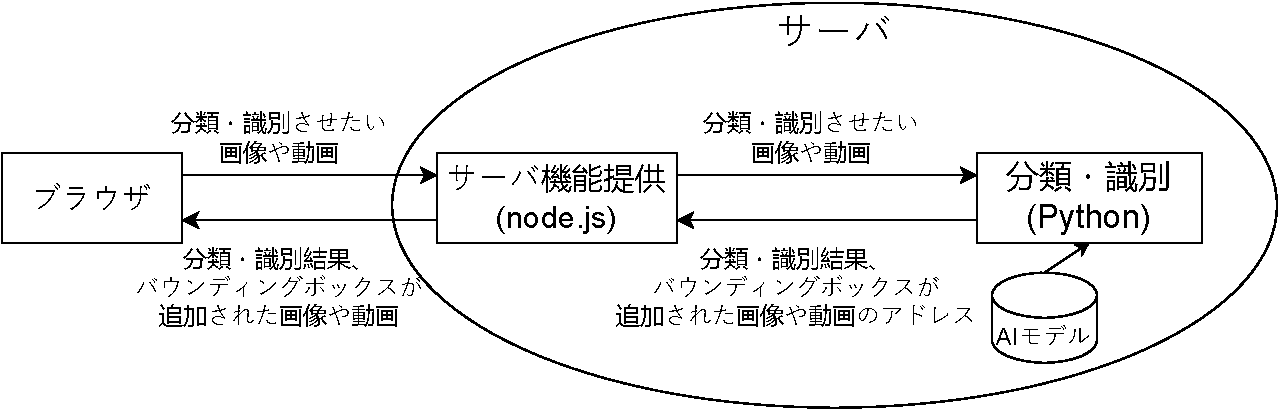
\includegraphics [width=\linewidth]{chap2/fig/sys_gaiyou6.pdf}
	\caption{システム概要図}
	\label{FIG}
\end{figure}

\section{システムの機能}
%本システムの機能として電車の分類と識別を提供する.識別は動画と画像の両方に対応している.
%画像や動画を入力すると,判別結果が出力される.
本システムは,以下の3つの機能を提供する.
%本システムは,電車の画像の分類と電車の画像と動画の識別の3つ機能を提供する
\begin{itemize}
	\item 電車の画像の分類
	\item 電車の画像の識別
	\item 電車の動画の識別
\end{itemize}

\subsection{電車の画像の分類} 
出力後の画面を図\ref{img_cls}に示す.
この機能では,ユーザがブラウザからアップロードした画像に含まれる電車の種類を分類する. 分類の結果,最も可能性が高いものをWebページに出力する.
\subsection{電車の画像の識別}
出力後の画面を図\ref{img_det}に示す.
この機能では,ユーザがブラウザからアップロードした画像に含まれる電車の位置と種類を識別する.  識別の結果,バウンディングボックスが追加された画像をWebページに表示する.
\subsection{電車の動画の識別} 
出力後の画面を図\ref{mov_det}に示す.
この機能では,ユーザがブラウザからアップロードした動画に含まれる電車の位置と種類を識別する. 識別の結果,バウンディングボックスが追加された動画をWebページに表示する.

%\begin{figure}
%	\centering
%	\includegraphics[width=0.5\linewidth]{obj/image1.png}
%	\figcap{画像の分類}{classify image}{cls-img}
%\end{figure}

\begin{figure}[H]
	\begin{tabular}{ccc}
		\begin{minipage}[b]{0.3\textwidth}
			\centering
			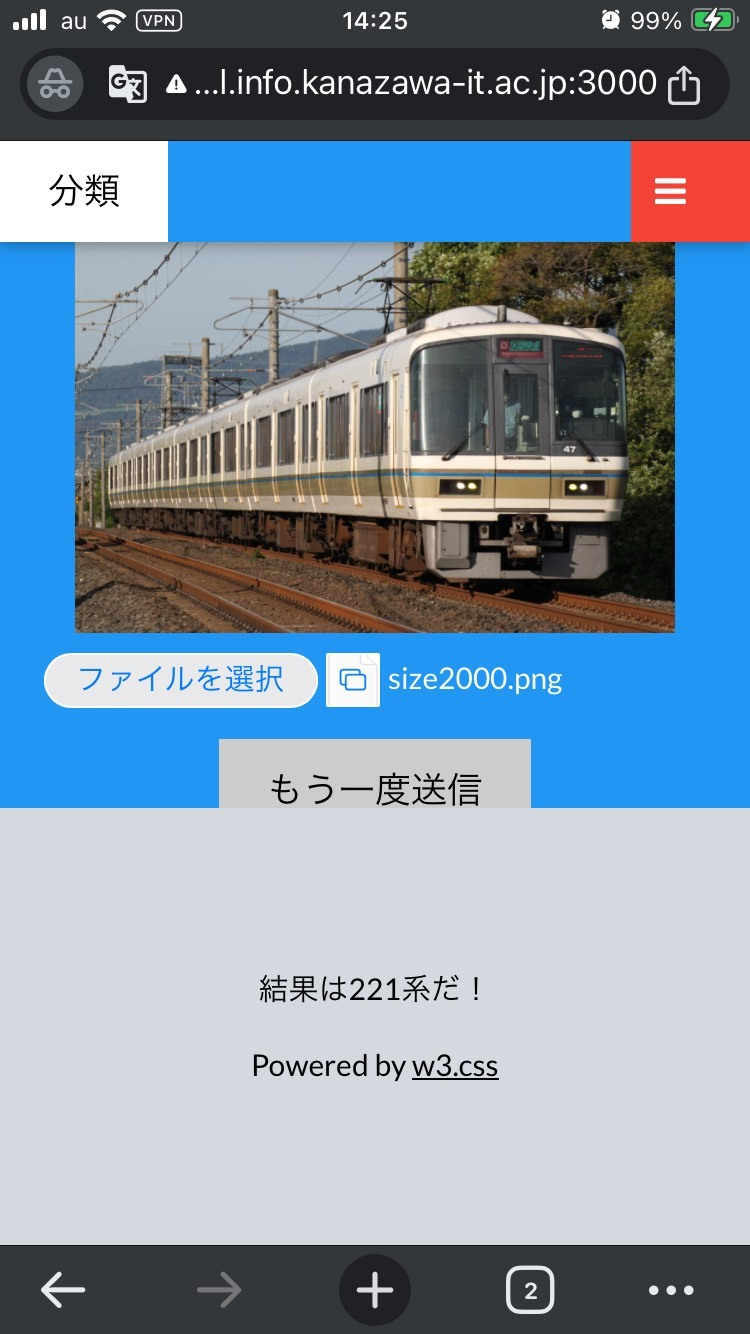
\includegraphics[width=\linewidth]{chap2/fig/img_classify.jpg}
			\caption{画像の分類}
			\label{img_cls}
		\end{minipage}
		\begin{minipage}[b]{0.3\textwidth}
			\centering
			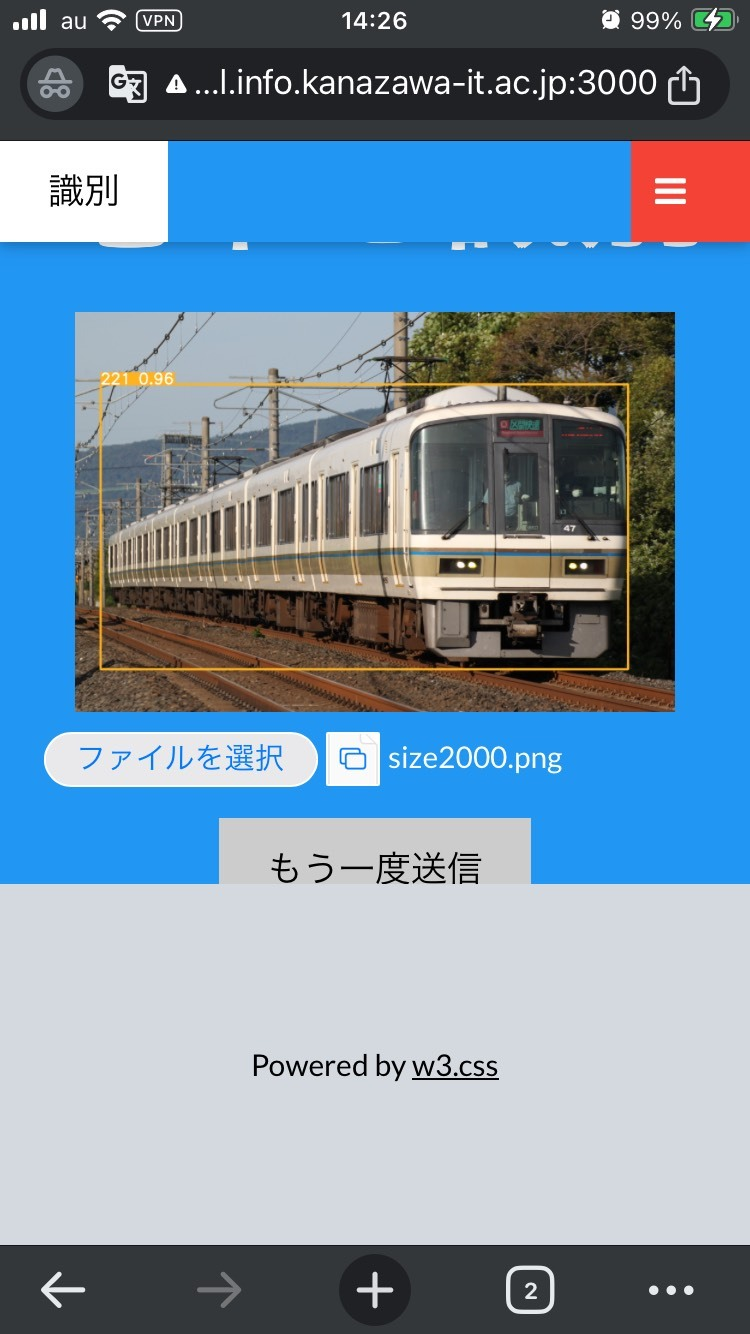
\includegraphics[width=\linewidth]{chap2/fig/img_identify.jpg}
			\caption{画像の識別}
			\label{img_det}
		\end{minipage}
		\begin{minipage}[b]{0.3\textwidth}
			\centering
			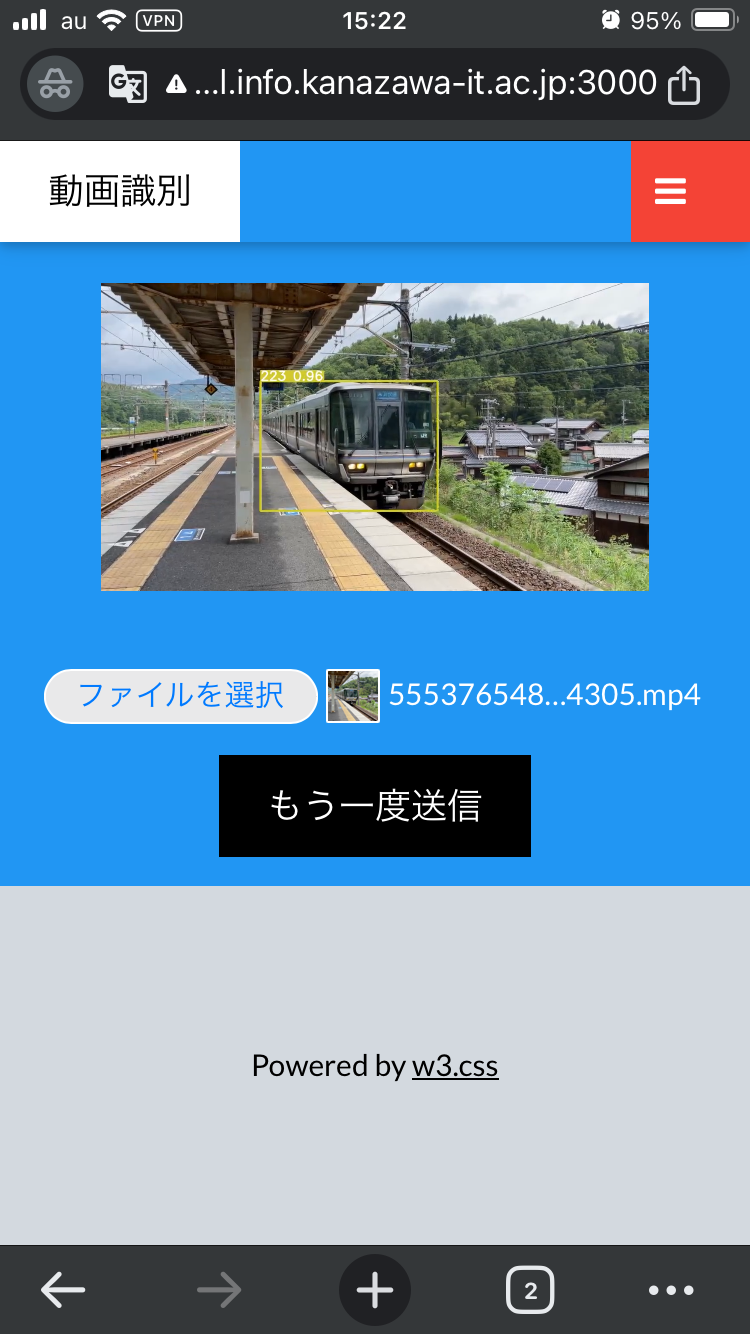
\includegraphics[width=\linewidth]{chap2/fig/mov_identify1.jpg}
			\caption{動画の識別}
			\label{mov_det}
		\end{minipage}
	\end{tabular}
\end{figure}



\section{動作環境}
アプリケーションを動作させるサーバ,学習を行う環境(?)として研究室で使用されているマシンを利用した.
サーバのスペックは以下の通りである.
\begin{itemize} 
	\item OS: Ubuntu 20.04.5 LTS 
	\item メモリ(RAM): 50GB 
	\item CPU: Intel(R) Core(TM) i7-8086K 
	\item コア数:6
	\item クロック周波数:4GHz
	\item キャッシュサイズ:12.288MB
	\item GPU: NVIDIA GeForce RTX 2080 Ti 
	\item HDD: 480GB 
	\item TPM: 2
	\item MTU(最大転送単位):1500
	\item RX(受信パケット): 78106237
	\item TX(送信パケット): 18475
\end{itemize}

最新の動作が確認されたテスト環境はChrome 120.0.6099.119である.



\section{使用言語}
Webアプリケーションに使用した言語はそれぞれ
フロントエンド
\begin{itemize}
	\item html
	\item JavaScript
	\item CSS
\end{itemize}
バックエンド
\begin{itemize}
	\item JavaScript(node.js)
	\item Python
\end{itemize}
である.

\section{デザイン,レイアウトについて}
デザインはレスポンシブデザインを意識して行った.
レイアウトは画面サイズに応じて,要素が横幅100%相対的または可変的に調整されたレイアウトであるリキッドレイアウトとなっている.
また,要素の数が少なく横に並べる必要が無いと判断したため,できる限り中央ぞろえで縦に要素を配置した.
PCで見たindex.htmlを\ref{fig_pc_index}に示す.
%参考 レスポンシブ,リキッドレイアウト,フレキシブルレイアウト,その他レスポンシブに関すること #HTML,CSS - Qiita
%https://qiita.com/yokomoji12345/items/f94ce43e9fd9b8637543
\section{使用したテンプレートについて}
テンプレートにはw3.schoolの出しているテンプレートを使用した.
%参考 W3.CSS Templates https://www.w3schools.com/w3css/w3css_templates.asp
元のテンプレートの見た目を\ref{fig_pc_template}に示す.

\begin{figure}[H]
	\begin{tabular}{cc}
		\begin{minipage}[b]{0.45\textwidth}
			\centering
			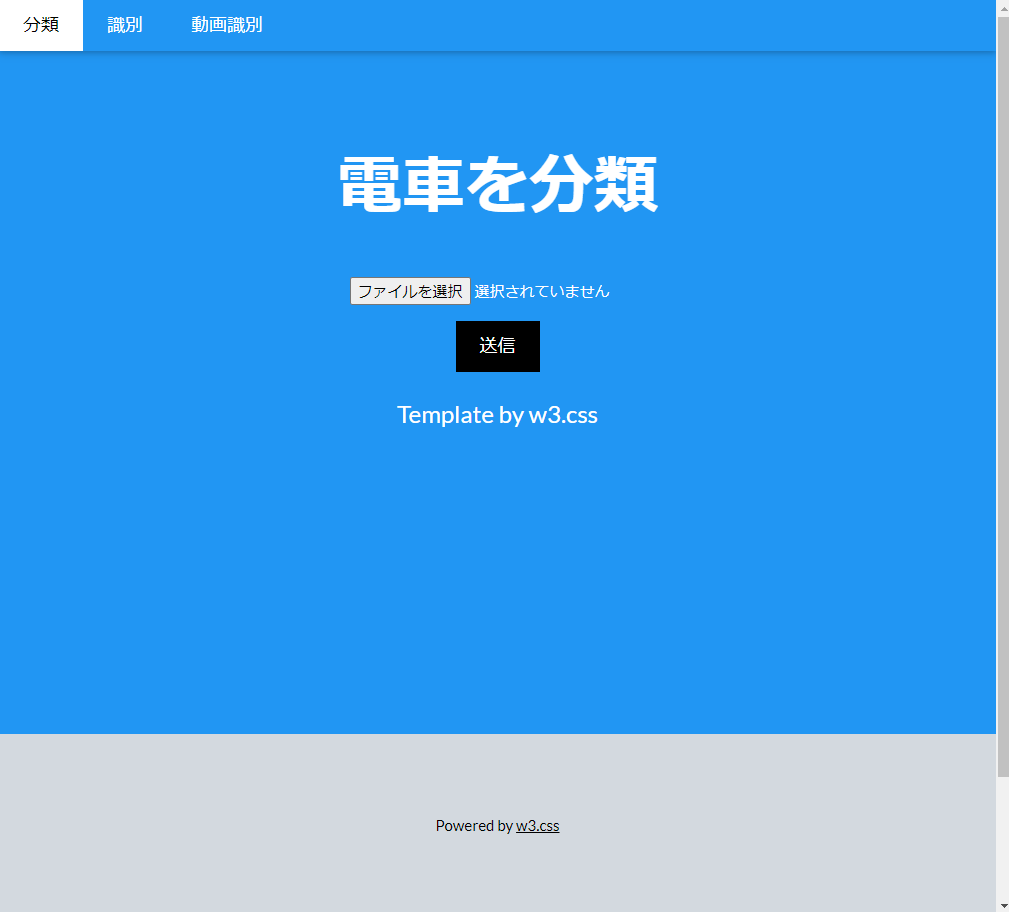
\includegraphics [width=\linewidth]{chap2/fig/pc_index.png}%配置するチャプターに応じて変えて
			\caption{PCで見た際のindex.html}	\label{fig_pc_index}
		\end{minipage}	
		\begin{minipage}[b]{0.45\textwidth}
			\centering
			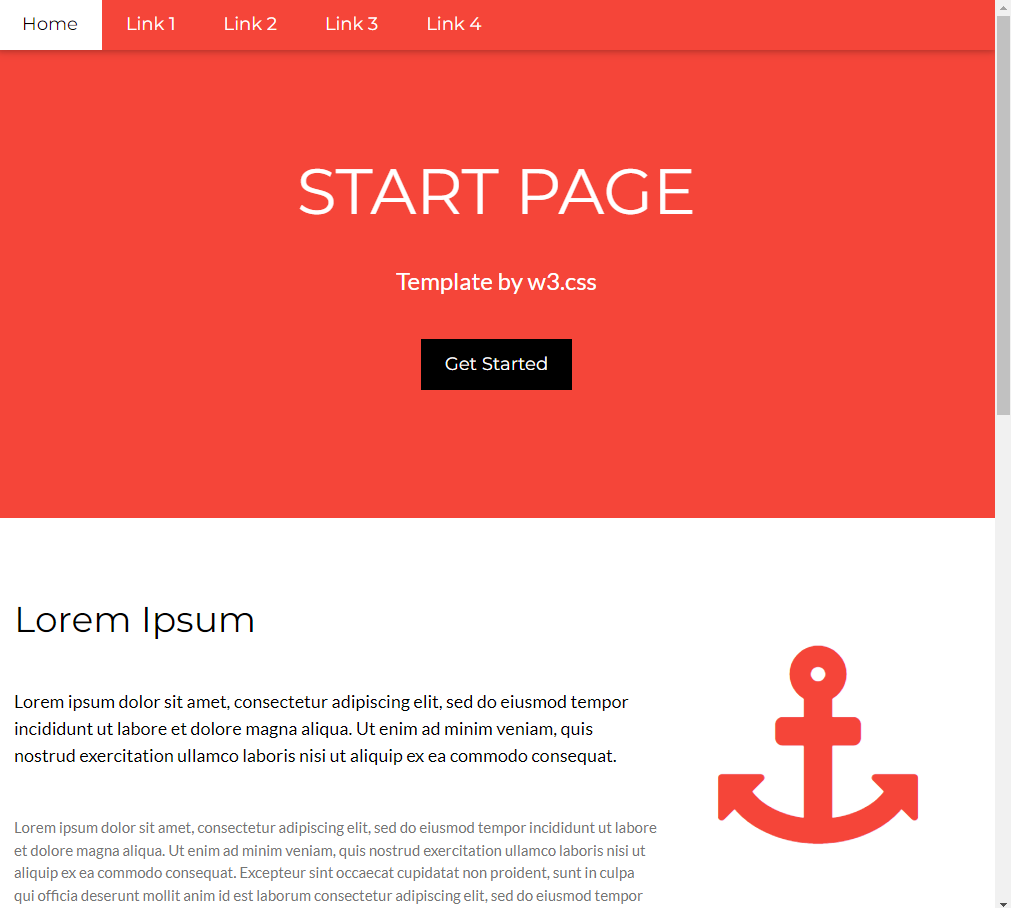
\includegraphics [width=\linewidth]{chap2/fig/pc_template.png}%配置するチャプターに応じて変えて
			\caption{テンプレートの見た目}\label{fig_pc_template}
		\end{minipage}
	\end{tabular}
\end{figure}



\section{動作確認と現状}
動作確認
 % 2章
% !TeX root = paper.tex


\chapter{学習データの準備}\label{genri}
%\section{この章で書くこと}
%\begin{itemize}
%	\item djangoの件
%	\item 電車が映っている場面だけ画像で保存
%	\item データセットを作成(識別・分類)
%	\item アノテーションについて
%\end{itemize}

\section{データの収集}
学習データは,車両タイプごとにその車両タイプが映っているYouTubeの動画をダウンロードして,任意の枚数分のランダムなフレームを保存する.その後,保存した画像を識別して電車が映っている画像を保存してレーニングデータとバリデーションデータを収集した.テストデータは様々なウェブサイトから手作業で17種類の各車両の画像を10枚ずつ収集した.
本プロジェクトでは,JR西日本の在来線の電車を識別または分類する.\\
205  207  213  221  223  225  227  271  281  283  285  287  321  323  381  521  683 \\
上記の17種類の画像を集める.
% TODO: \usepackage{graphicx} required

\begin{figure}[htbp]
	\begin{tabular}{cc}
	\begin{minipage}[b]{0.15\linewidth}
			\centering
			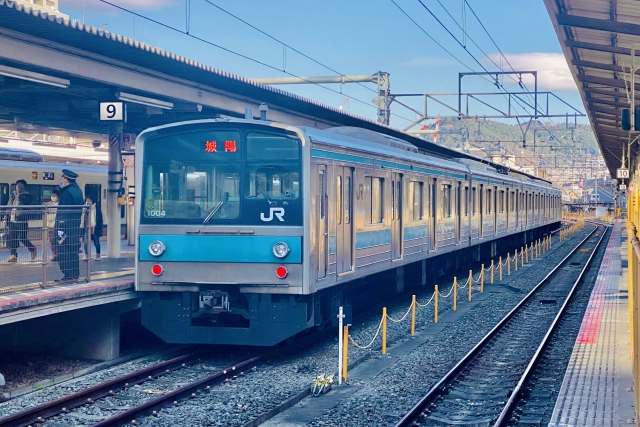
\includegraphics[width=\linewidth]{densya/205.jpg}
			\caption{205系}
			\label{fig:205}
	\end{minipage}
	\begin{minipage}[b]{0.15\textwidth}
		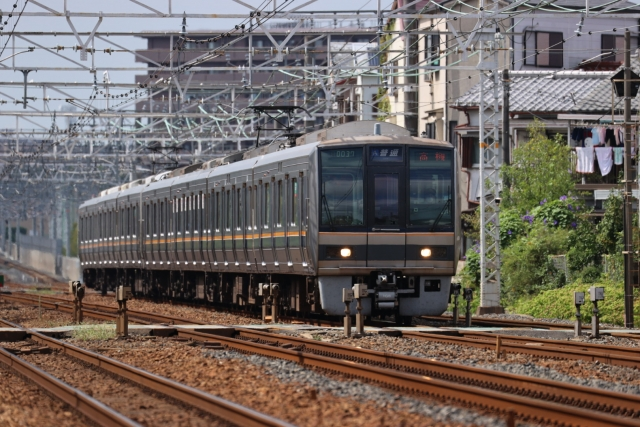
\includegraphics[width=\linewidth]{densya/207.jpg}
		\caption{207系}
		\label{fig:207}
	\end{minipage}
	\begin{minipage}[b]{0.15\textwidth}
		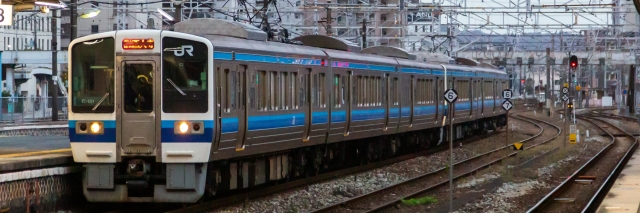
\includegraphics[width=\linewidth]{densya/213.jpg}
		\caption{213系}
		\label{fig:213}
	\end{minipage}
	\begin{minipage}[b]{0.15\textwidth}
		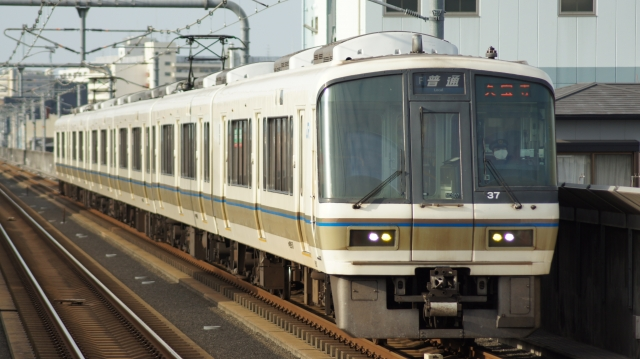
\includegraphics[width=\linewidth]{densya/221.jpg}
		\caption{221系}
		\label{fig:221}
	\end{minipage}
	\begin{minipage}[b]{0.15\textwidth}
		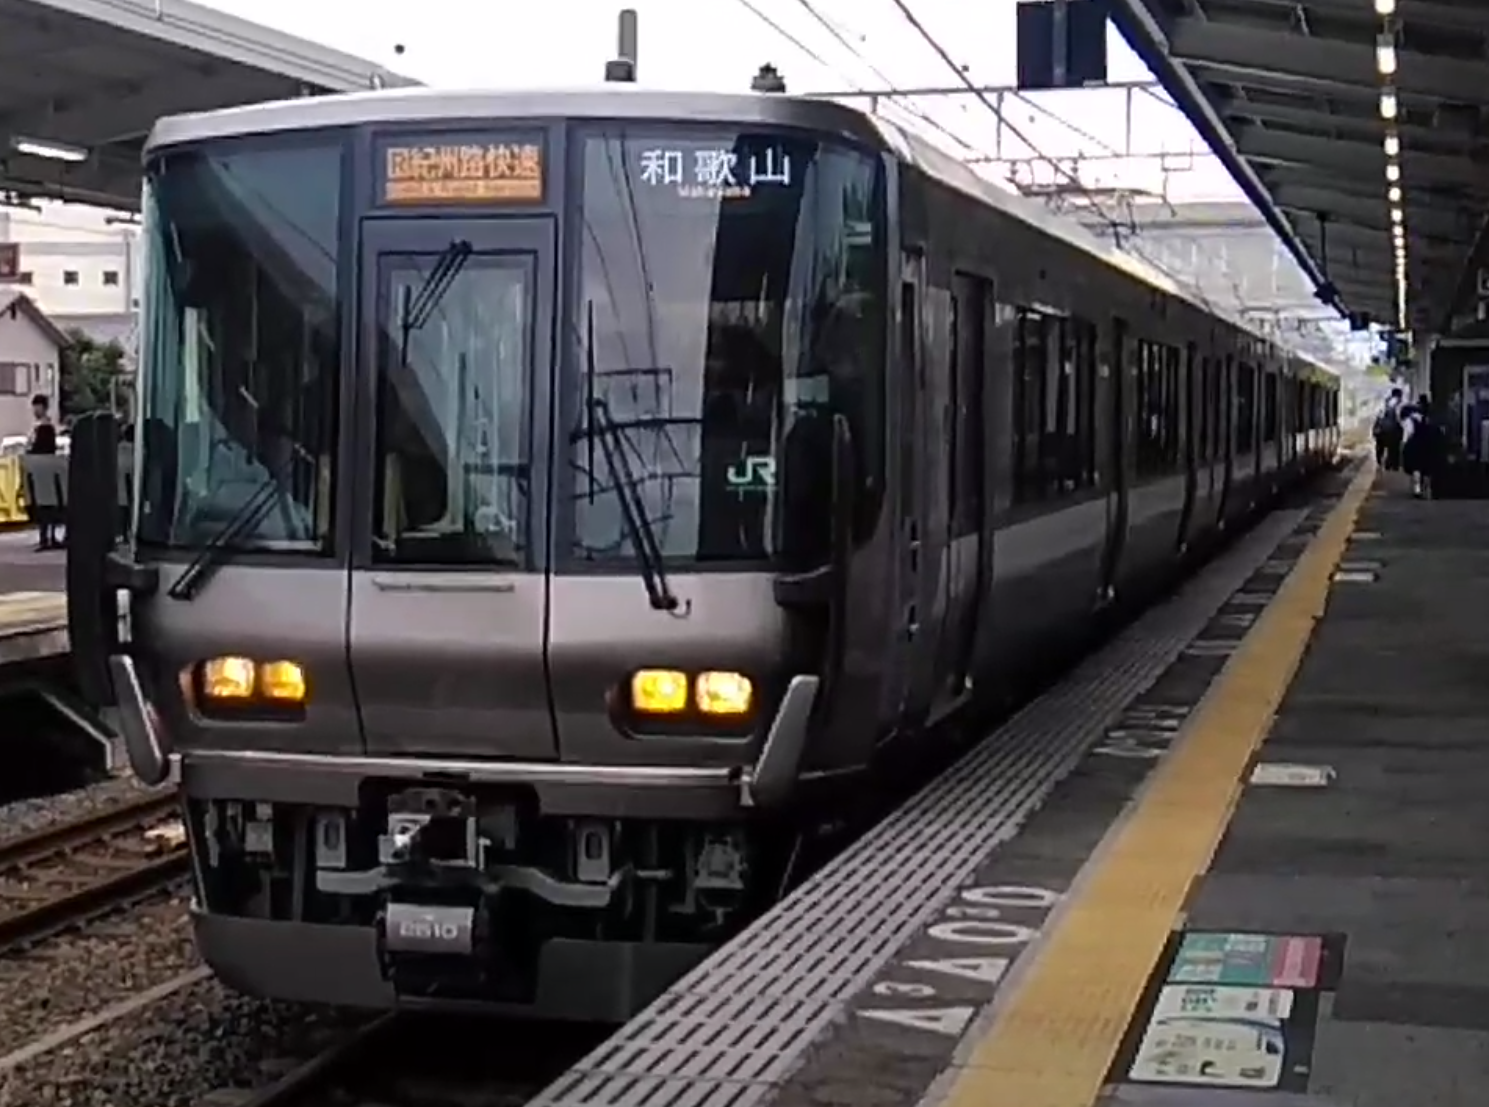
\includegraphics[width=\linewidth]{densya/223.png}
		\caption{223系}
		\label{fig:223}
	\end{minipage}
	\begin{minipage}[b]{0.15\textwidth}
		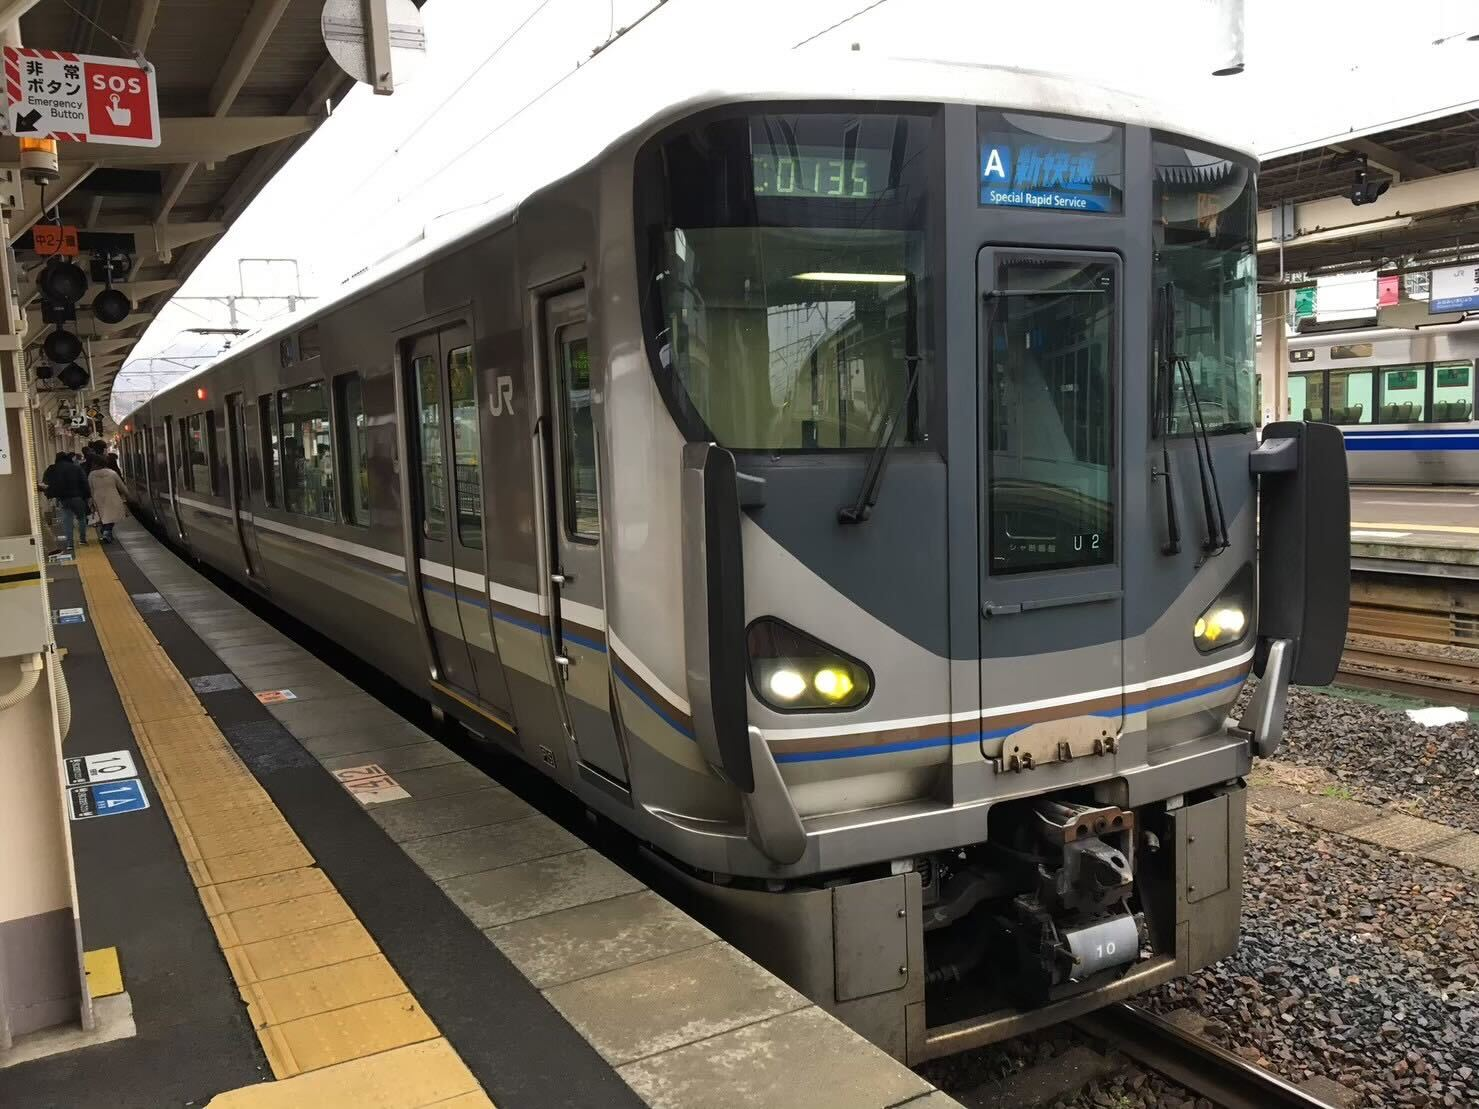
\includegraphics[width=\linewidth]{densya/225.jpg}
		\caption{225}
		\label{fig:225}
	\end{minipage}
	\end{tabular}
\end{figure}

\begin{figure}[htbp]
	\begin{tabular}{cc}
		\begin{minipage}[b]{0.15\linewidth}
			\centering
			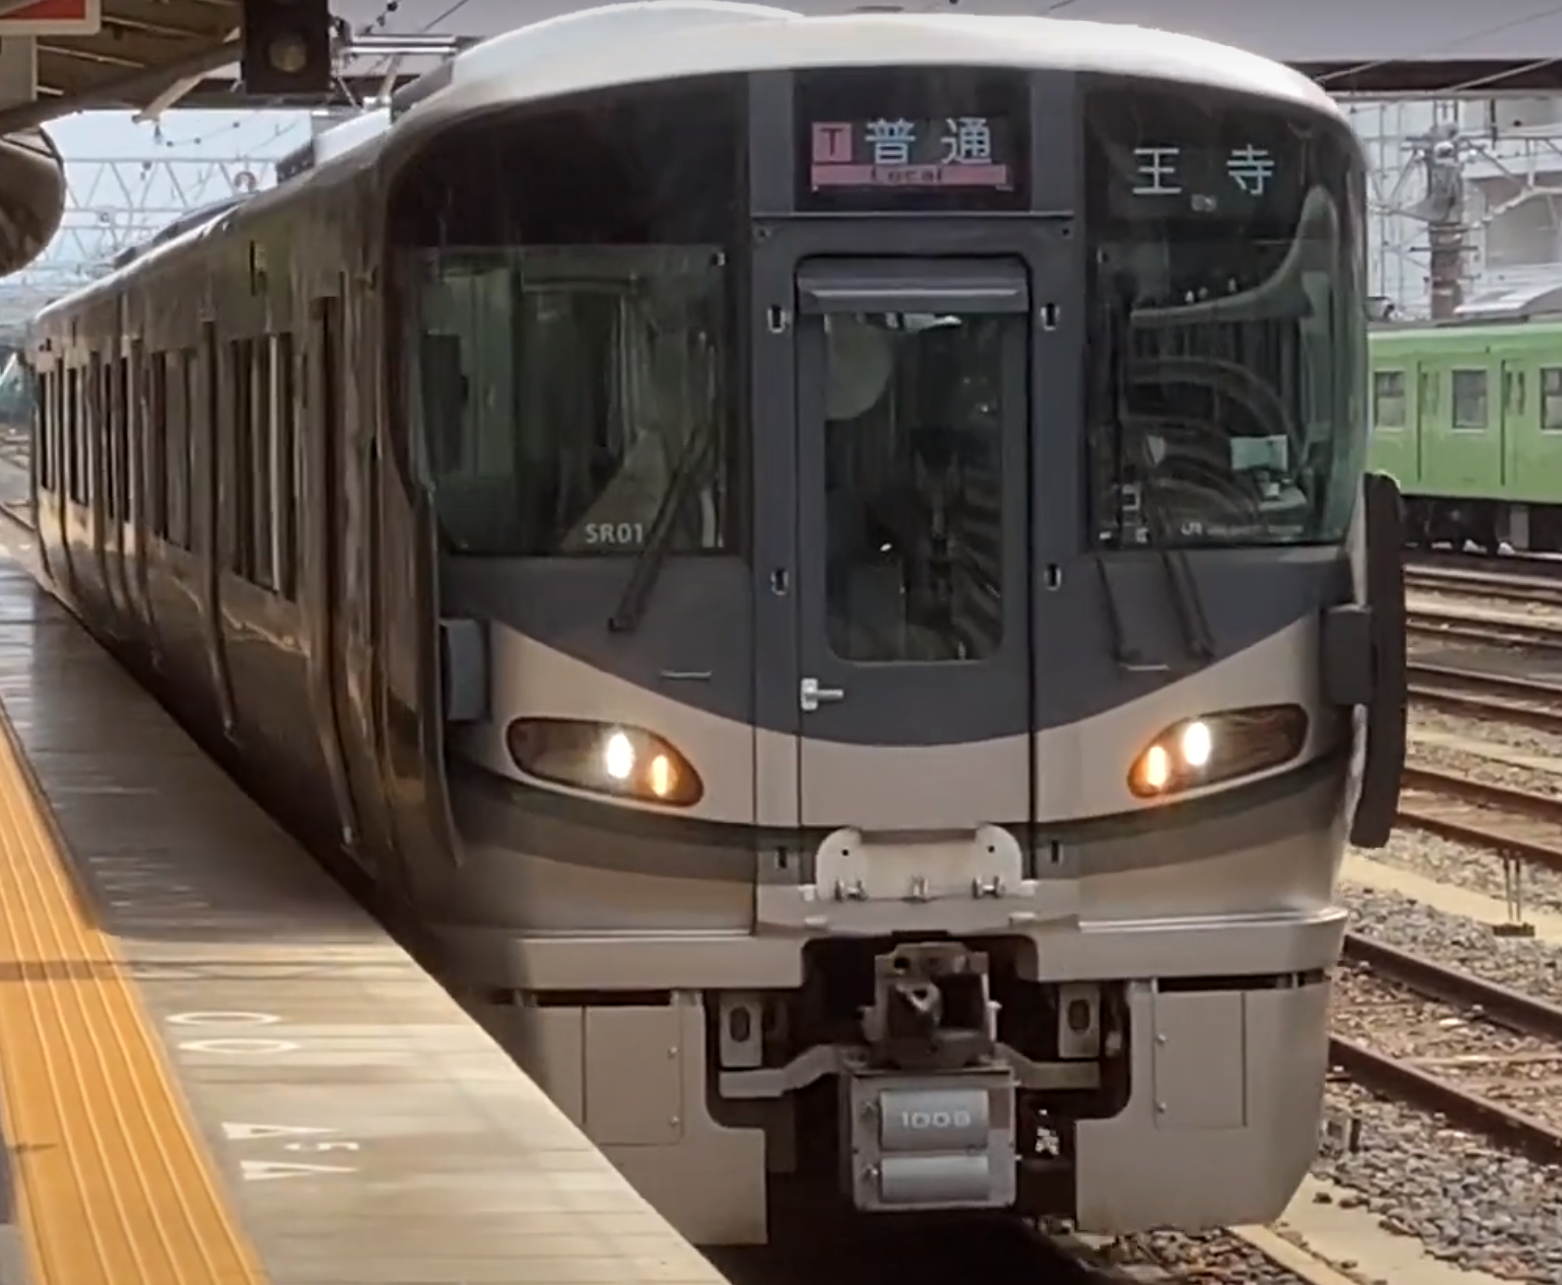
\includegraphics[width=\linewidth]{densya/227.png}
			\caption{227系}
			\label{fig:227}
		\end{minipage}
		\begin{minipage}[b]{0.15\textwidth}
			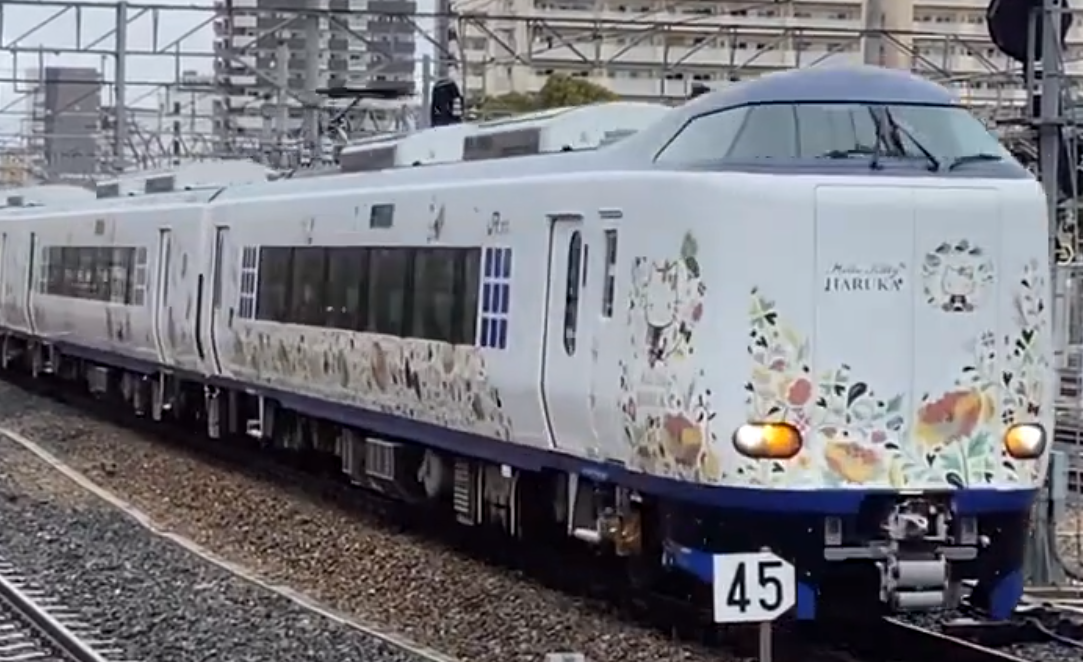
\includegraphics[width=\linewidth]{densya/271.png}
			\caption{271系}
			\label{fig:271}
		\end{minipage}
		\begin{minipage}[b]{0.15\textwidth}
			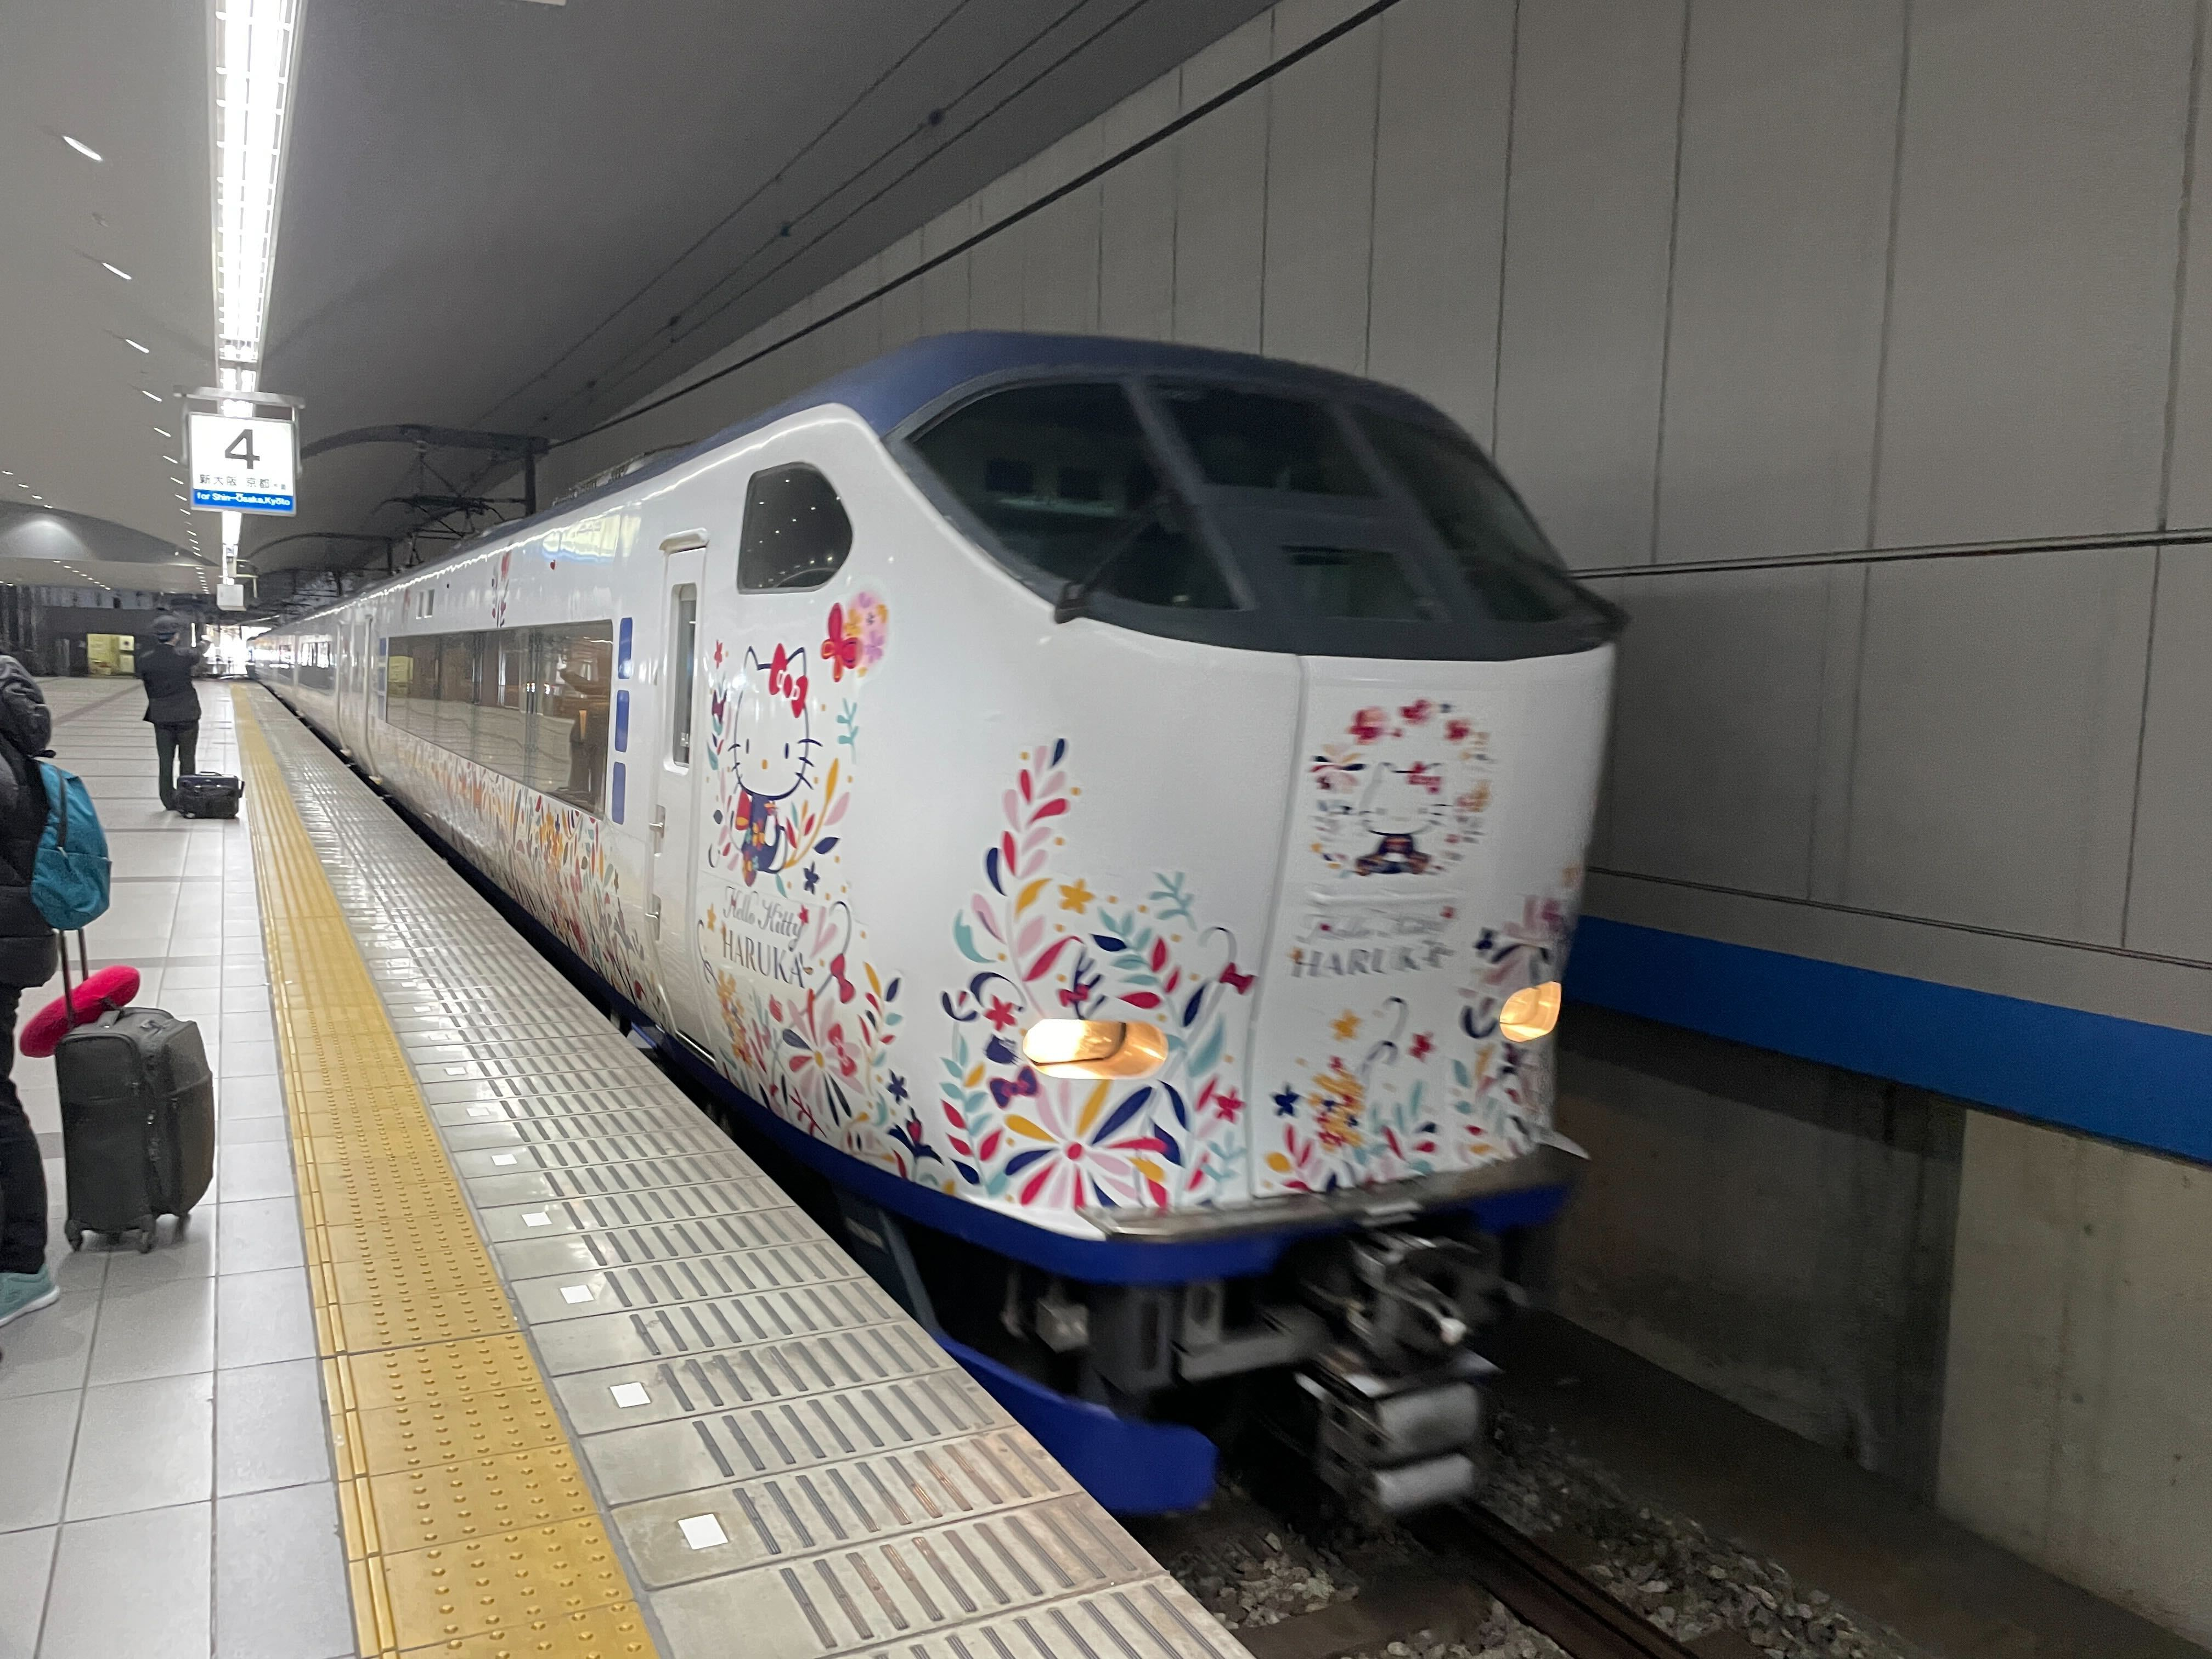
\includegraphics[width=\linewidth]{densya/281.jpg}
			\caption{281系}
			\label{fig:281}
		\end{minipage}
	\begin{minipage}[b]{0.15\textwidth}
		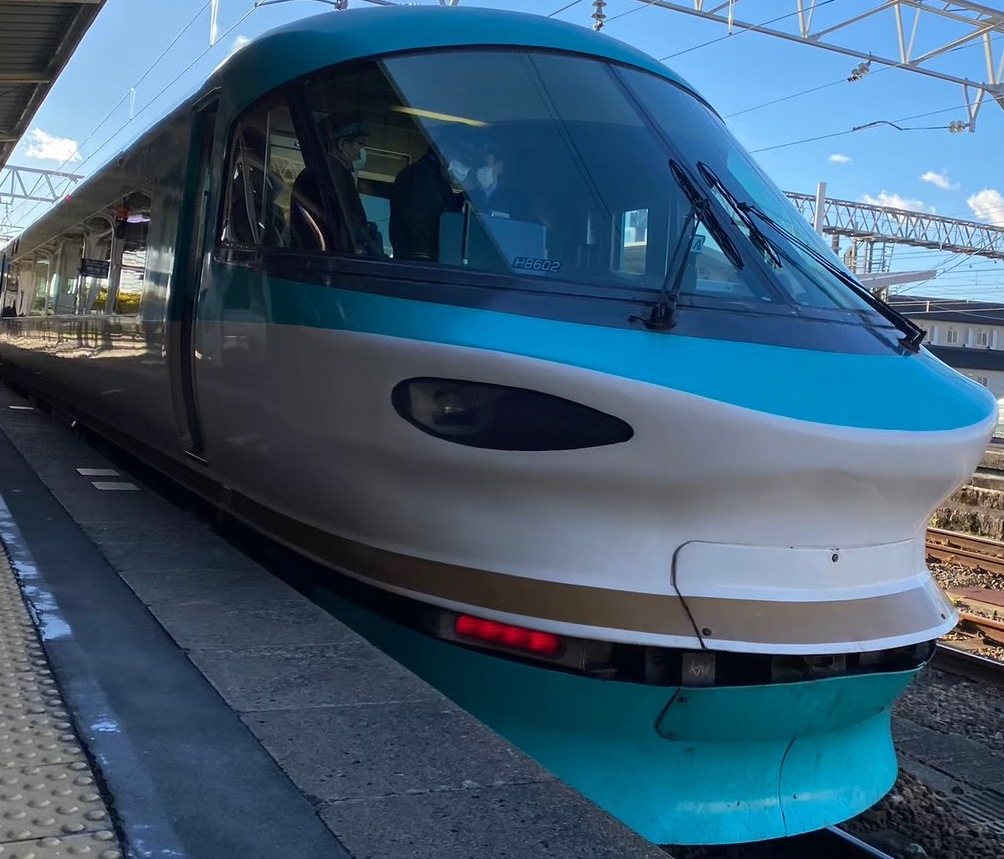
\includegraphics[width=\linewidth]{densya/283.jpg}
		\caption{283系}
		\label{fig:283}
	\end{minipage}
		\begin{minipage}[b]{0.15\textwidth}
			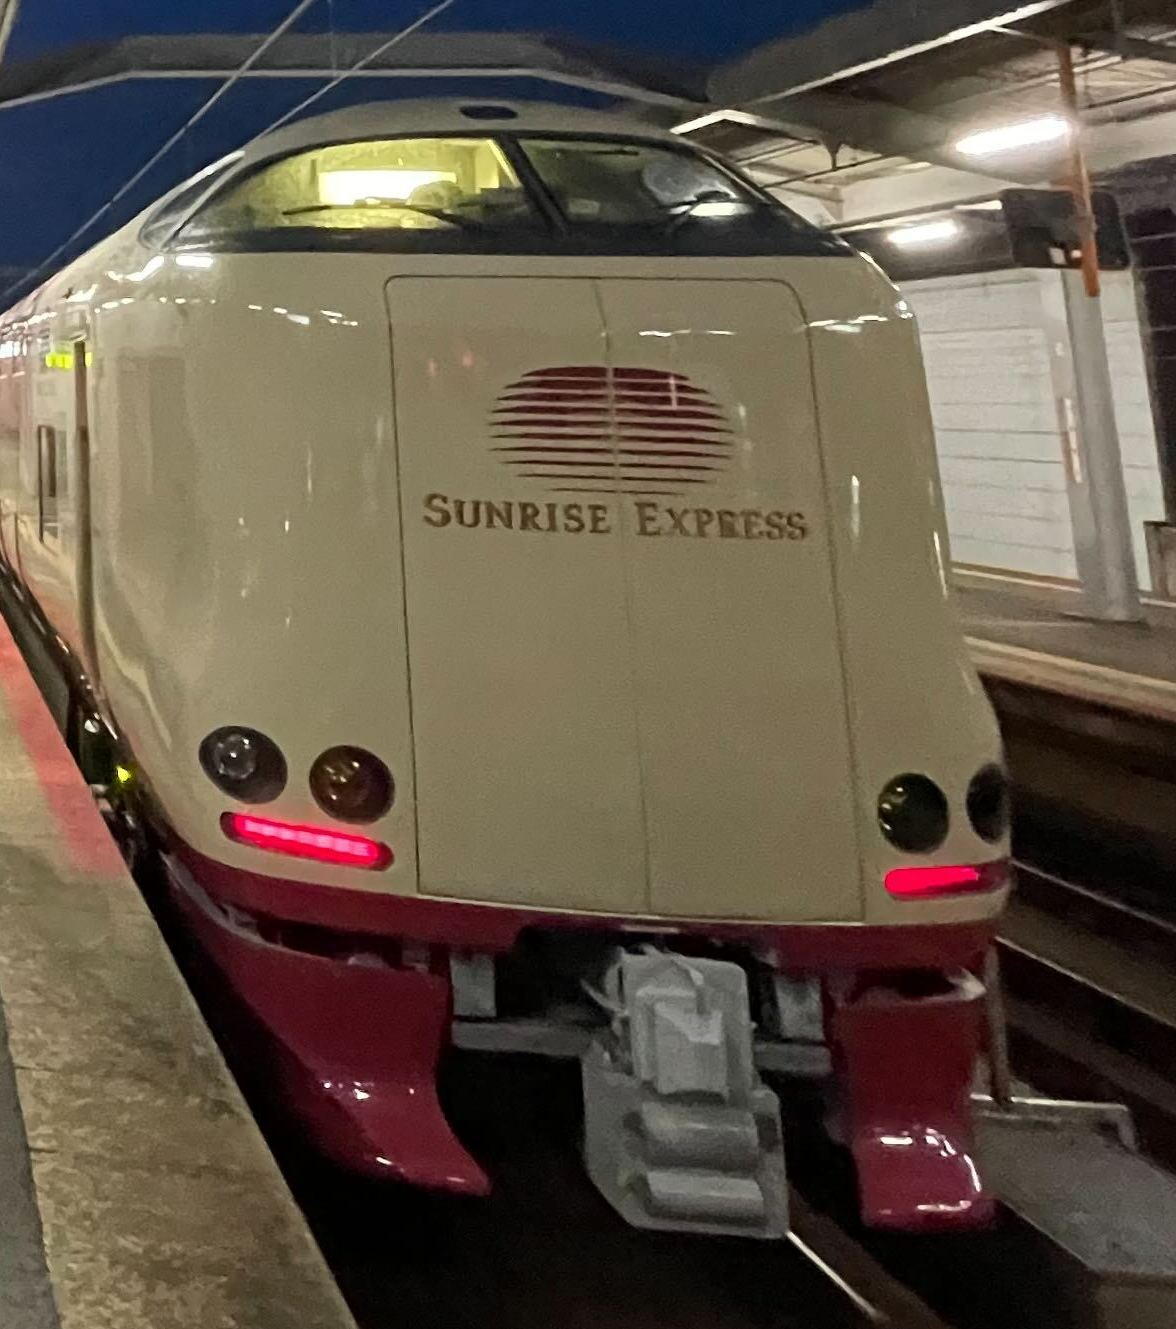
\includegraphics[width=\linewidth]{densya/285.jpg}
			\caption{285系}
			\label{fig:285}
		\end{minipage}
		\begin{minipage}[b]{0.15\textwidth}
			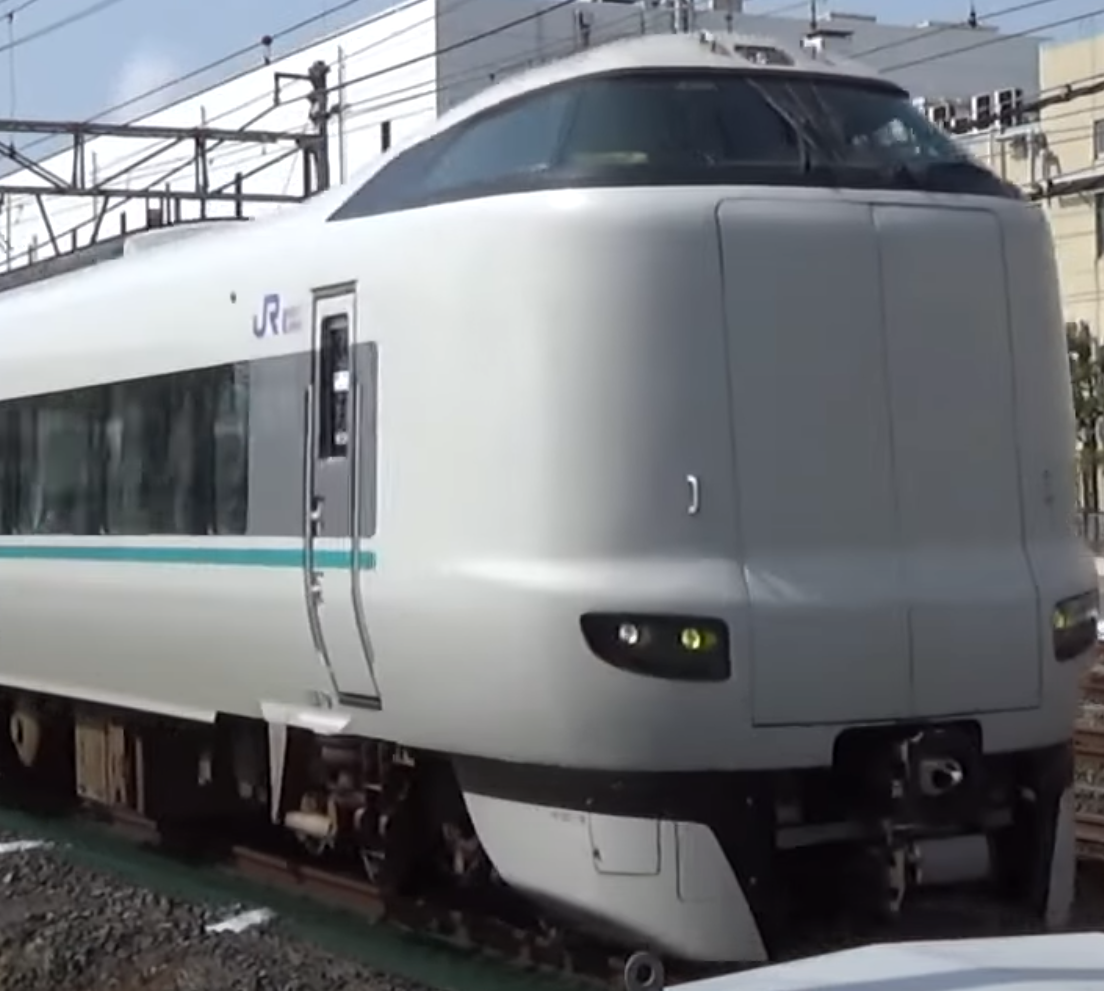
\includegraphics[width=\linewidth]{densya/287.png}
			\caption{287系}
			\label{fig:287}
		\end{minipage}
	
	\end{tabular}
\end{figure}

\begin{figure}[htbp]
	\begin{tabular}{cc}
		\begin{minipage}[b]{0.15\textwidth}
			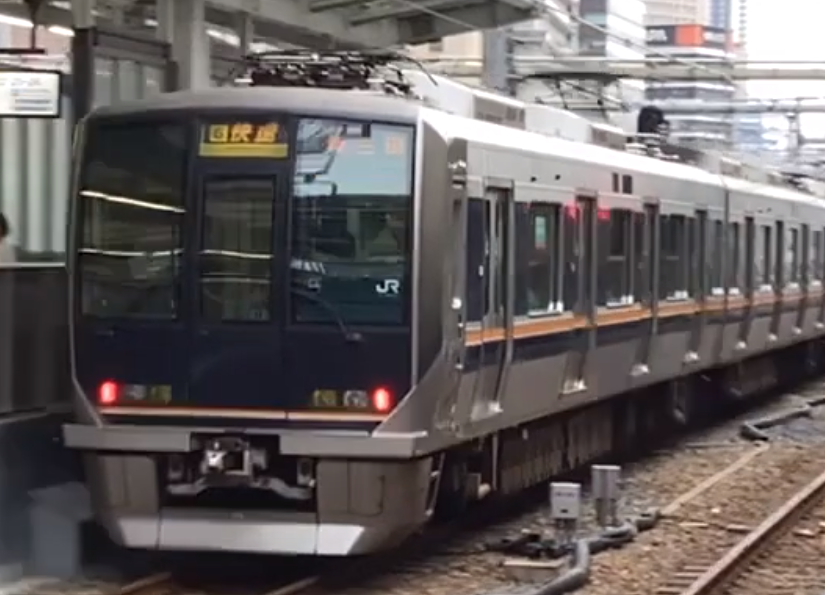
\includegraphics[width=\linewidth]{densya/321.png}
			\caption{321系}
			\label{fig:321}
		\end{minipage}
		\begin{minipage}[b]{0.15\linewidth}
			\centering
			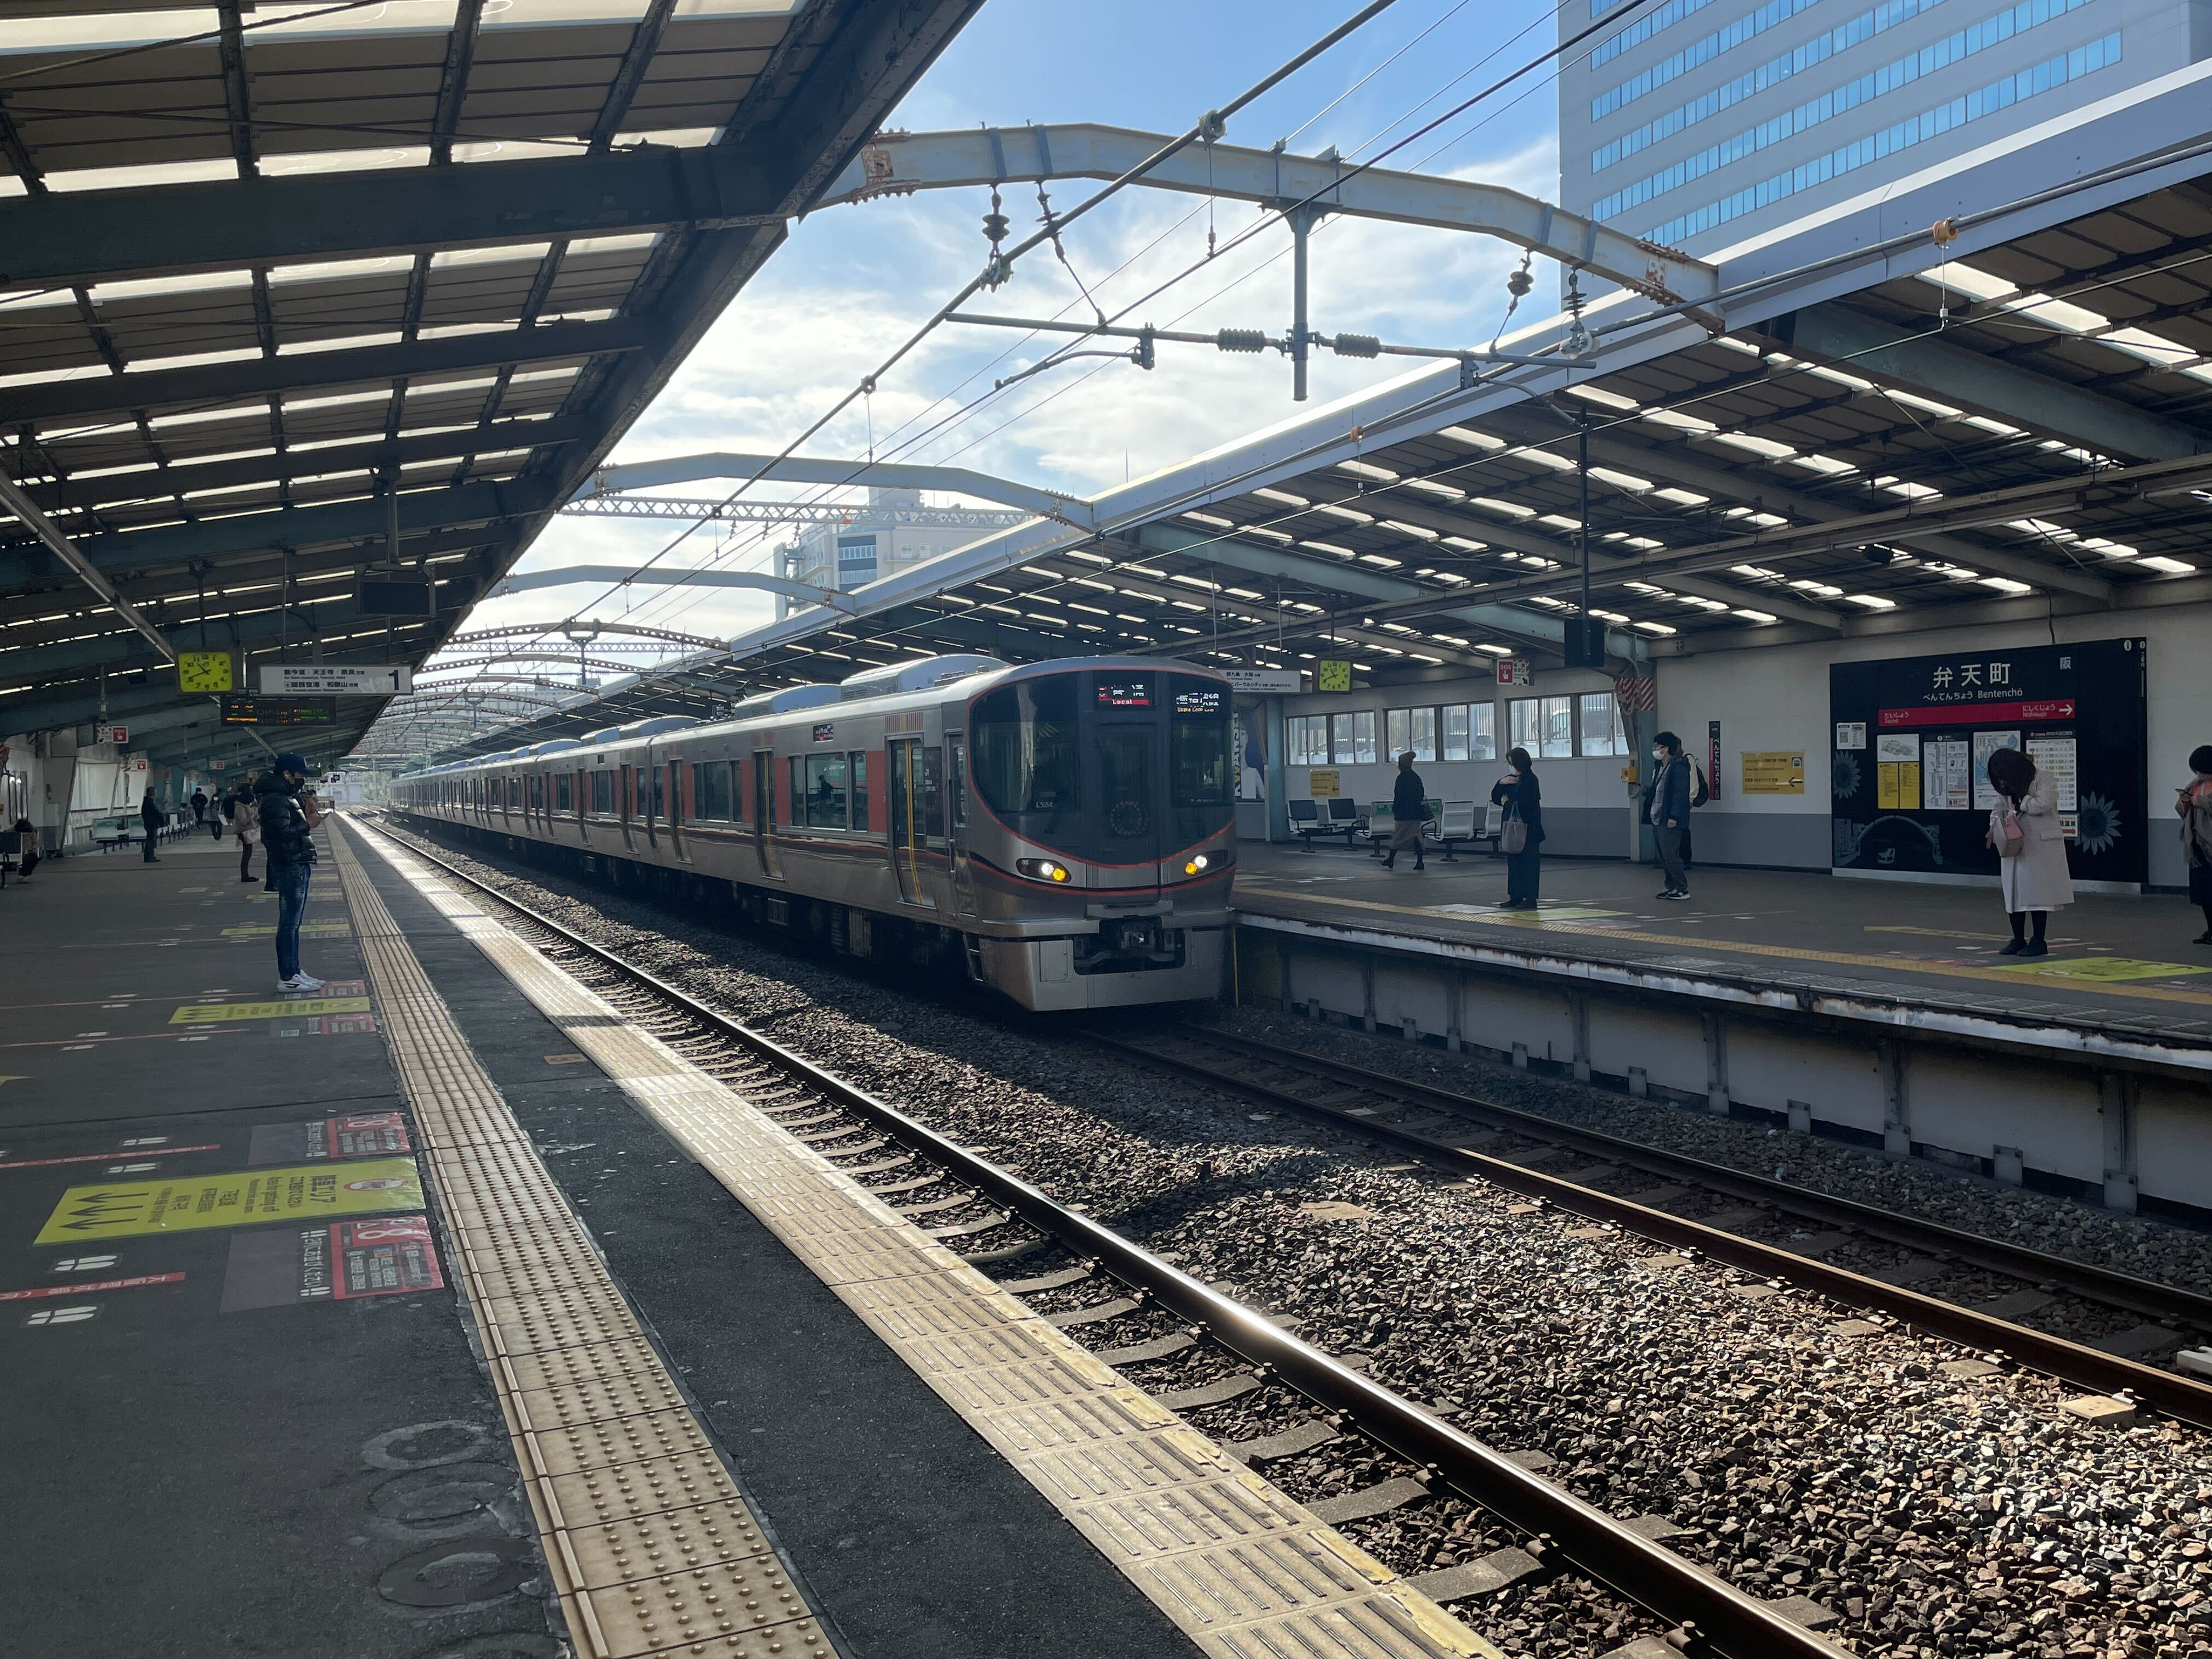
\includegraphics[width=\linewidth]{densya/323.jpg}
			\caption{323系}
			\label{fig:323}
		\end{minipage}
		\begin{minipage}[b]{0.15\textwidth}
			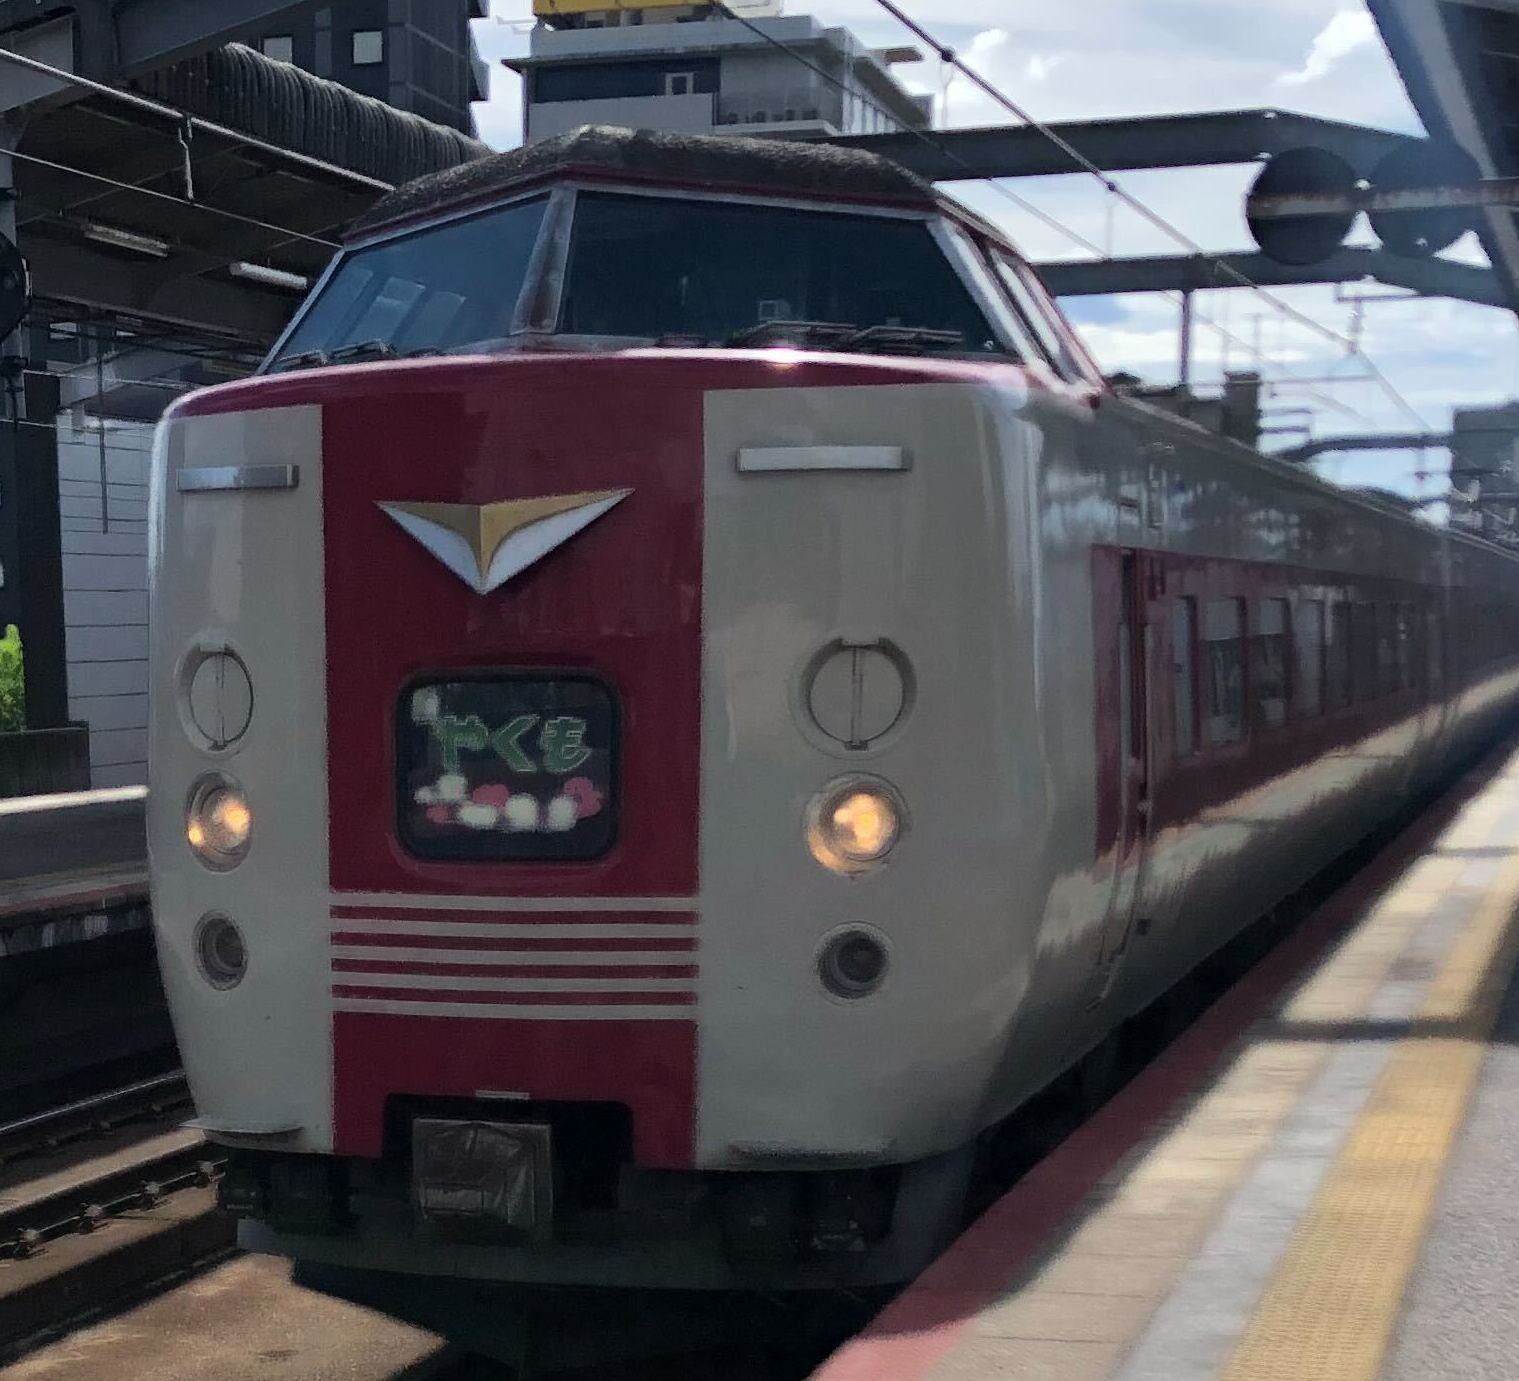
\includegraphics[width=\linewidth]{densya/381.jpg}
			\caption{381系}
			\label{fig:381}
		\end{minipage}
		\begin{minipage}[b]{0.15\textwidth}
			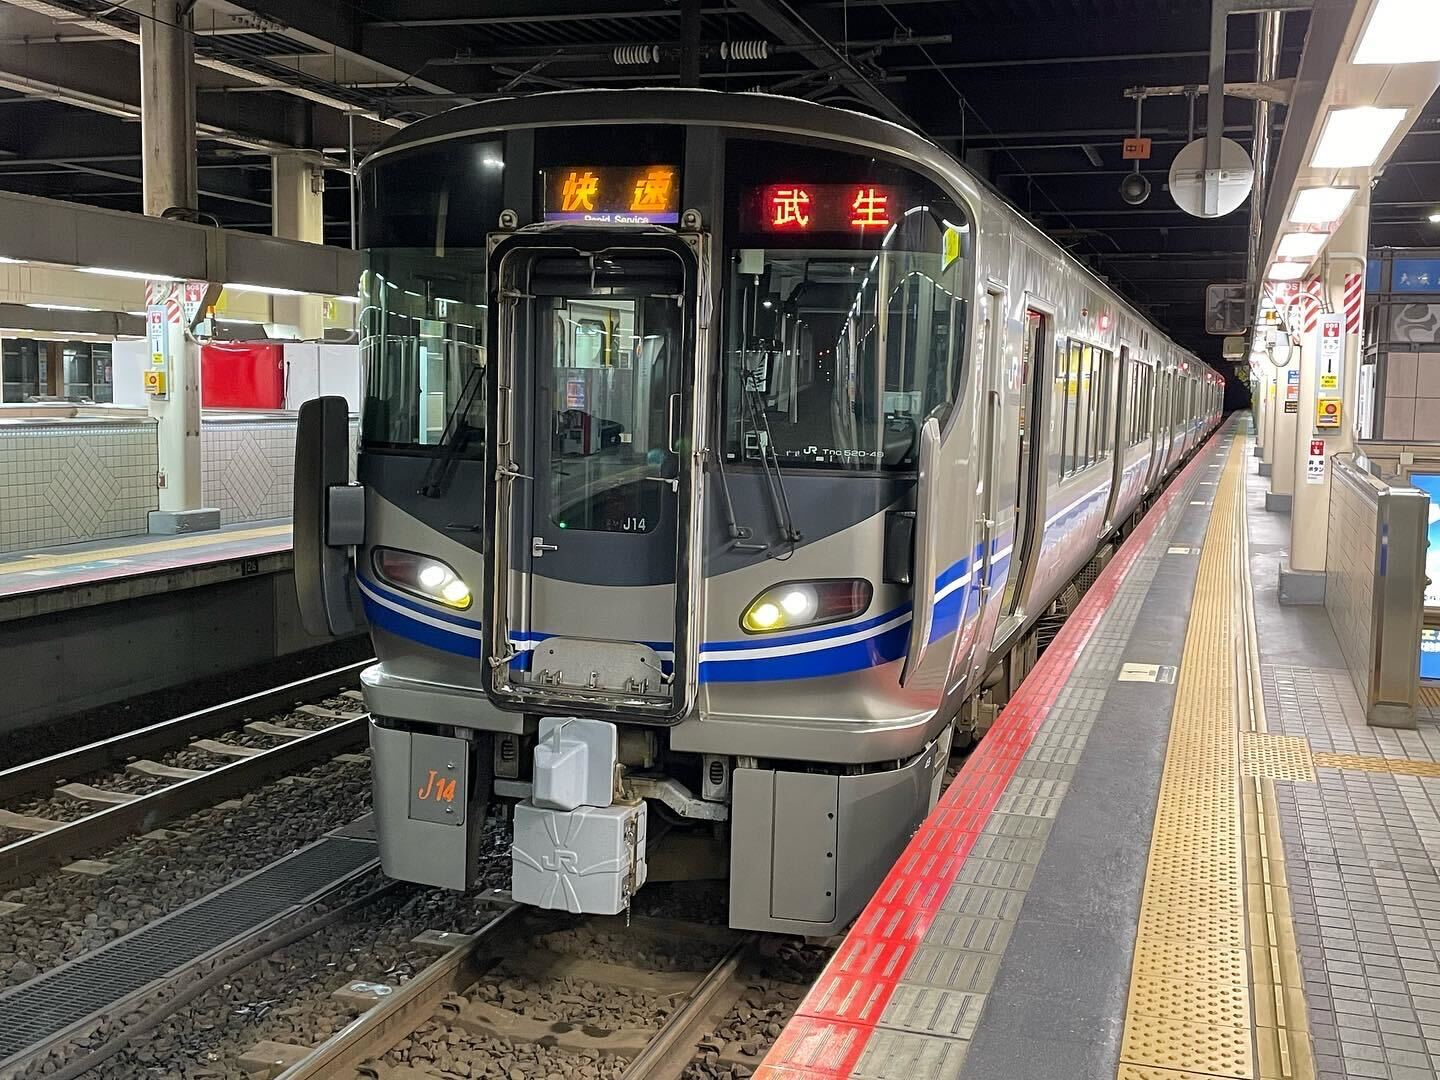
\includegraphics[width=\linewidth]{densya/521.jpg}
			\caption{521系}
			\label{fig:521}
		\end{minipage}
		\begin{minipage}[b]{0.15\textwidth}
			\includegraphics[width=\linewidth]{densya/683.jpg}
			\caption{683系}
			\label{fig:683}
		\end{minipage}
	\end{tabular}
\end{figure}


\subsection{動画の連結と保存}
動画の保存にはyt-dlpという動画や音声をダウンロードするプログラムを使う.
1〜3種類の動画の任意の秒数をダウンロードしてそれぞれの動画を連結して一つの動画にするwebアプリケーションをPythonのフレームワークの一つであるDjangoを使って作成した.
%	\red{画像は後で変える,大きさを揃える}\\
	作成したwebアプリケーションは,図\ref{test3}のようになっている.
	YouTube上の動画のURLと開始時刻(秒),終了時刻(秒),車両タイプ名を入力して,1〜3種類の動画を保存し連結して一つの動画にしている.
	
\begin{figure}[H]
	\includegraphics [width=0.9\linewidth]{chap3/fig/test3.png}
	\caption{動画のダウンロード3,あとで画像を差し替え}
	\label{test3}
\end{figure}

\subsection{画像の保存}
保存した動画を利用して指定した枚数分のランダムなフレームを保存する.保存した画像を識別し電車が映っている画像だけを保存す,トレーニングデータとバリデーションデータを収集した.
テストデータは様々なウェブサイトから手作業で17種類の各車両の画像を10枚ずつ収集した.
車両タイプごとに保存した画像の枚数を図\ref{fig:chart}に示す.

% TODO: \usepackage{graphicx} required

% TODO: \usepackage{graphicx} required
\begin{figure}[H]
	\centering
	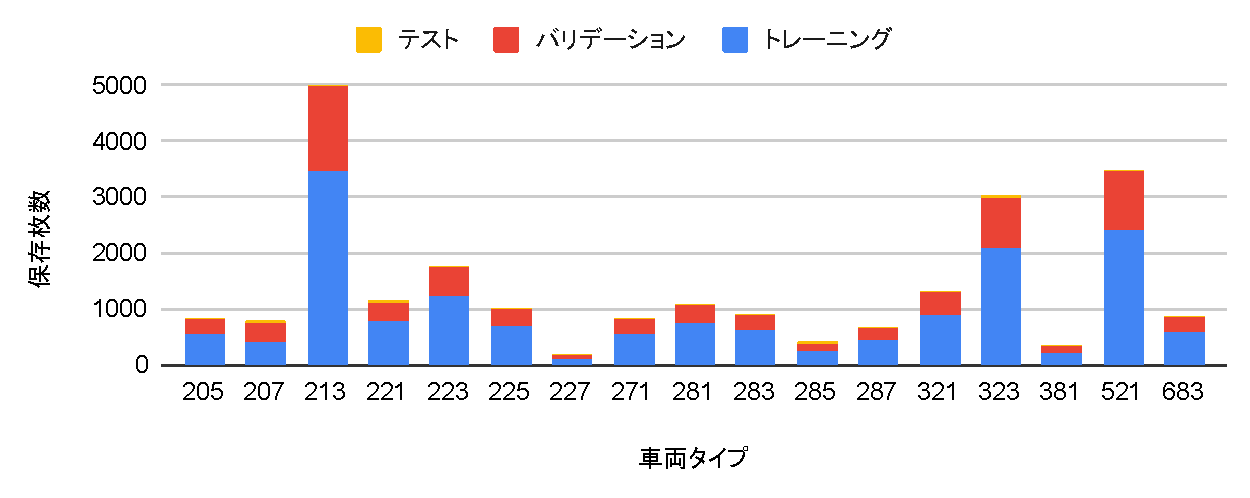
\includegraphics[width=\linewidth]{chap3/fig/chart2}
	\caption{各車両タイプ(全17種)の保存枚数}
	\label{fig:chart}
\end{figure}



\section{データセットの作成}
%\subsection{データセットの構造}

識別モデル用データセットと分類モデル用データセットの学習時に使用する画像は同じものを使う.識別モデル用のデータセットには画像のアノテーション情報が必要なので,アノテーションも行った.
このテストデータセットと作成したモデルを使って分類または識別を行い,モデルの性能の評価を行う.
%\subsection{アノテーション}
%https://www.dir.co.jp/world/entry/solution/annotation
アノテーションとは、機械学習の分類の一つである教師あり学習において,分析対象データにラベルを付与するプロセスである.画像にバウンディングボックスと呼ばれる四角形を描画しクラス番号を指定する.バウンディングボックスを描画することでその画像に写っている物体の座標情報を取得することができる.クラス番号とは,判別したいものリストを作成し,画像に写っている物体に対応した,リストのインデックスのことである.アノテーションをした結果は,識別モデルの学習時に使用する.

一般的にアノテーションは,手作業で行うものである.
しかし,数千枚の画像を手作業で行うことは難しいので,自動で行えるようにした.
分類モデル用のデータセットでは一枚の画像に電車が一つだけ映っている.その画像を配布されている識別用モデルで識別することでクラス番号と電車が映っている座標情報をテキストに書き込む.その後,本プロジェクトで識別する車両タイプリストに対応するクラス番号を上書きすることで,分類モデル用のデータセットから識別モデル用のデータセットを作成した.

 % 3章
% !TeX root = paper.tex


\chapter{車両タイプ判別モデルについて}
%\section{この章で書くこと}
%\begin{itemize}
%	\item 学習の実行
%	\item 性能評価
%	\item 作成したモデルの使い方
%	\item 出力されるものについて
%\end{itemize}


\section{学習の実行}
作成したデータセットとYOLOv8を用いてモデルの学習を行い,分類用と識別用の2種類のモデルを作成した.
分類モデルでは静止画での判別しかできない.動画から車両タイプを判別するために識別モデルを作成した.


\section{作成したモデルの使い方}
識別モデルと分類モデルで使い方はほぼ同じである.
作成したモデルをロードして,モデルに画像または動画を渡すと識別または分類をすることができる.\\
識別
\begin{verbatimx}
	from ultralytics import YOLO
	model = YOLO("作成した識別モデルのパス")
	results = model.predict("画像または動画のパス")
\end{verbatimx}

分類
\begin{verbatimx}
	from ultralytics import YOLO
	model = YOLO("作成した分類モデルのパス")
	results = model("画像のパス")
\end{verbatimx}

\section{出力されるもの}
17種類の車両が各10枚ずつ,合計170枚のテストデータセットを識別した際にターミナルに出力されるものを図 \ref{output}に示す.
左端のimageから,「何枚目か」「画像のパス」「入力画像のサイズ」「予想クラス番号」「予想クラス番号に対応する車両タイプ」「識別にかかった時間」が画像ごとに出力される.
識別時にsave = Trueを追加すると入力画像に識別結果が追記された画像が出力される.
識別時にsave\_txt = Trueを追加すると画像ごとに予想クラスと座標情報がテキストファイルで出力される.
モデルを動かした際に端末に出力されるものを図\ref{output}に記す.
\begin{figure}	
	\centering
	\includegraphics[width=\linewidth]{fig/a.pdf}
	\caption{端末に出力されるもの}\label{output}
\end{figure}

\section{作成したモデルの評価と考察}

\subsection{分類モデルの評価}
%分類モデルの評価を図\ref{CLS}に示す
\begin{figure}	
	\centering
	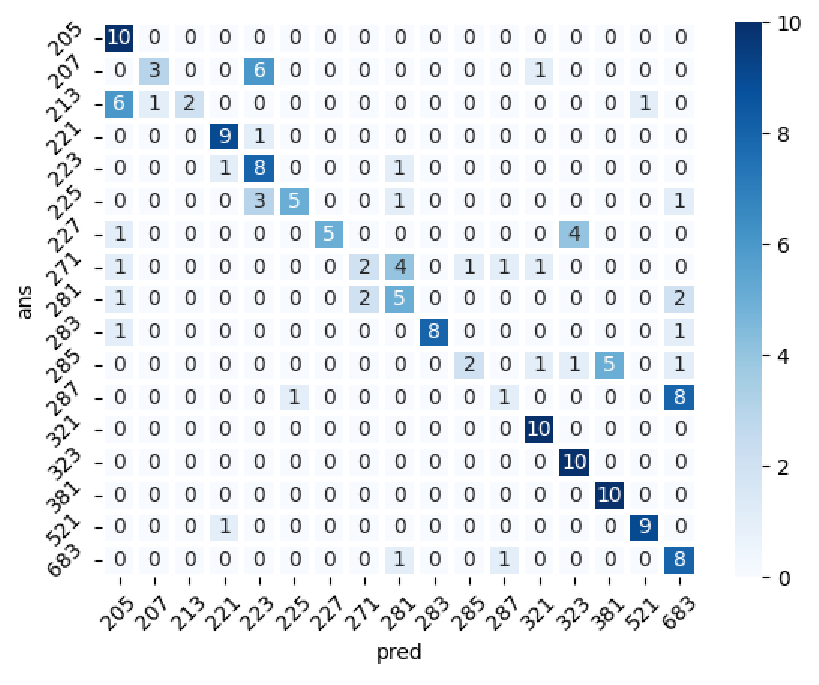
\includegraphics[width=\linewidth]{chap4/fig/classify_results.pdf}
	\caption{分類モデルの混合行列}
	\label{CLS}
\end{figure}
作成した分類モデルを用いてテストデータセットの分類を行った結果をを図\ref{CLS}に示す.
縦軸が予測した車両タイプ,横軸が正解の車両タイプとするグラフである.


\subsection{識別モデルの評価}
識別時には,どの車両タイプにも当てはまらないと識別されることがある.その場合の車両タイプは0として識別モデルの混合行列を作成した.
識別結果を表\ref{fig:chartdet} に示す.\\
%NaNとは識別成功数または識別失敗数が0のときに,IoUの平均が出せない場合の値である.\\
% TODO: \usepackage{graphicx} required
\begin{figure}[H]
	\centering
	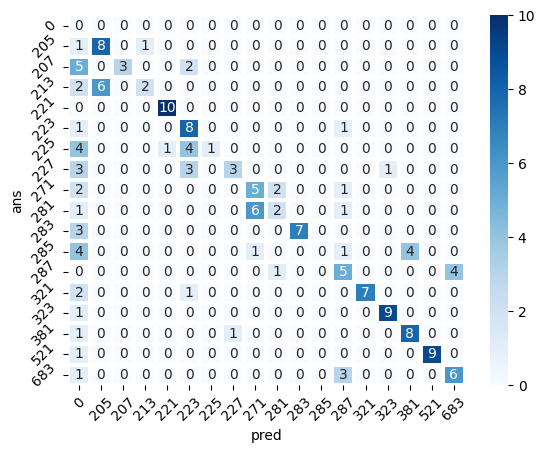
\includegraphics[width=\linewidth]{chap4/fig/predicted_results.jpg}
	\caption{識別モデルの混合行列}
	\label{fig:chartdet}
\end{figure}



\subsection{考察}
正解率は車両タイプによって異なることがわかる.287系と683系のように外見が似ている電車だと,誤判別していることが多かった.
287系を図\ref{fig:287},683系を図\ref{fig:683}に示す.
%データセットの画質を落とすと誤判別が増えた.特に誤分類が多かった三種類の電車の画質を上げても結果はあまり変わらなかった.
%限られたストレージでは,データセットの画質を変化させて判別結果を向上させることは難しいと考えられる.SSDの容量に制限がない場合,大量の高画質のデータでデータセットを作成することで判別結果が改善される可能性があると考えられる.
%各車両タイプの画像の枚数に差があったことが判別結果に影響を与えていると考えられる.
データセットの画像の枚数が少ない車両タイプの判別結果が必ず悪くはならなかった.
画像の枚数が判別結果に影響を与えるのではなく,車体の特徴が鮮明に写っている画像の枚数が判別結果に影響を与えると考えられる.
判別精度の向上のために,データセットとして質の悪い画像を大量に集めるのではなく,車体の特徴が鮮明に写っている画像を車両タイプごとに集める必要があったと考えられる.

同じ画像を使って,分類用と識別用の2種類のデータセットを作成した.分類モデルの混合行列と識別モデルの混合行列が似ているため,車両タイプを知るためのシステムを作る際には,識別モデルのみを作成することで画像と動画の両方に対応した車両判別システムを作成でき,電車の車両タイプを知ることができるようになると考える.

% TODO: \usepackage{graphicx} required
\begin{figure}
	\centering
	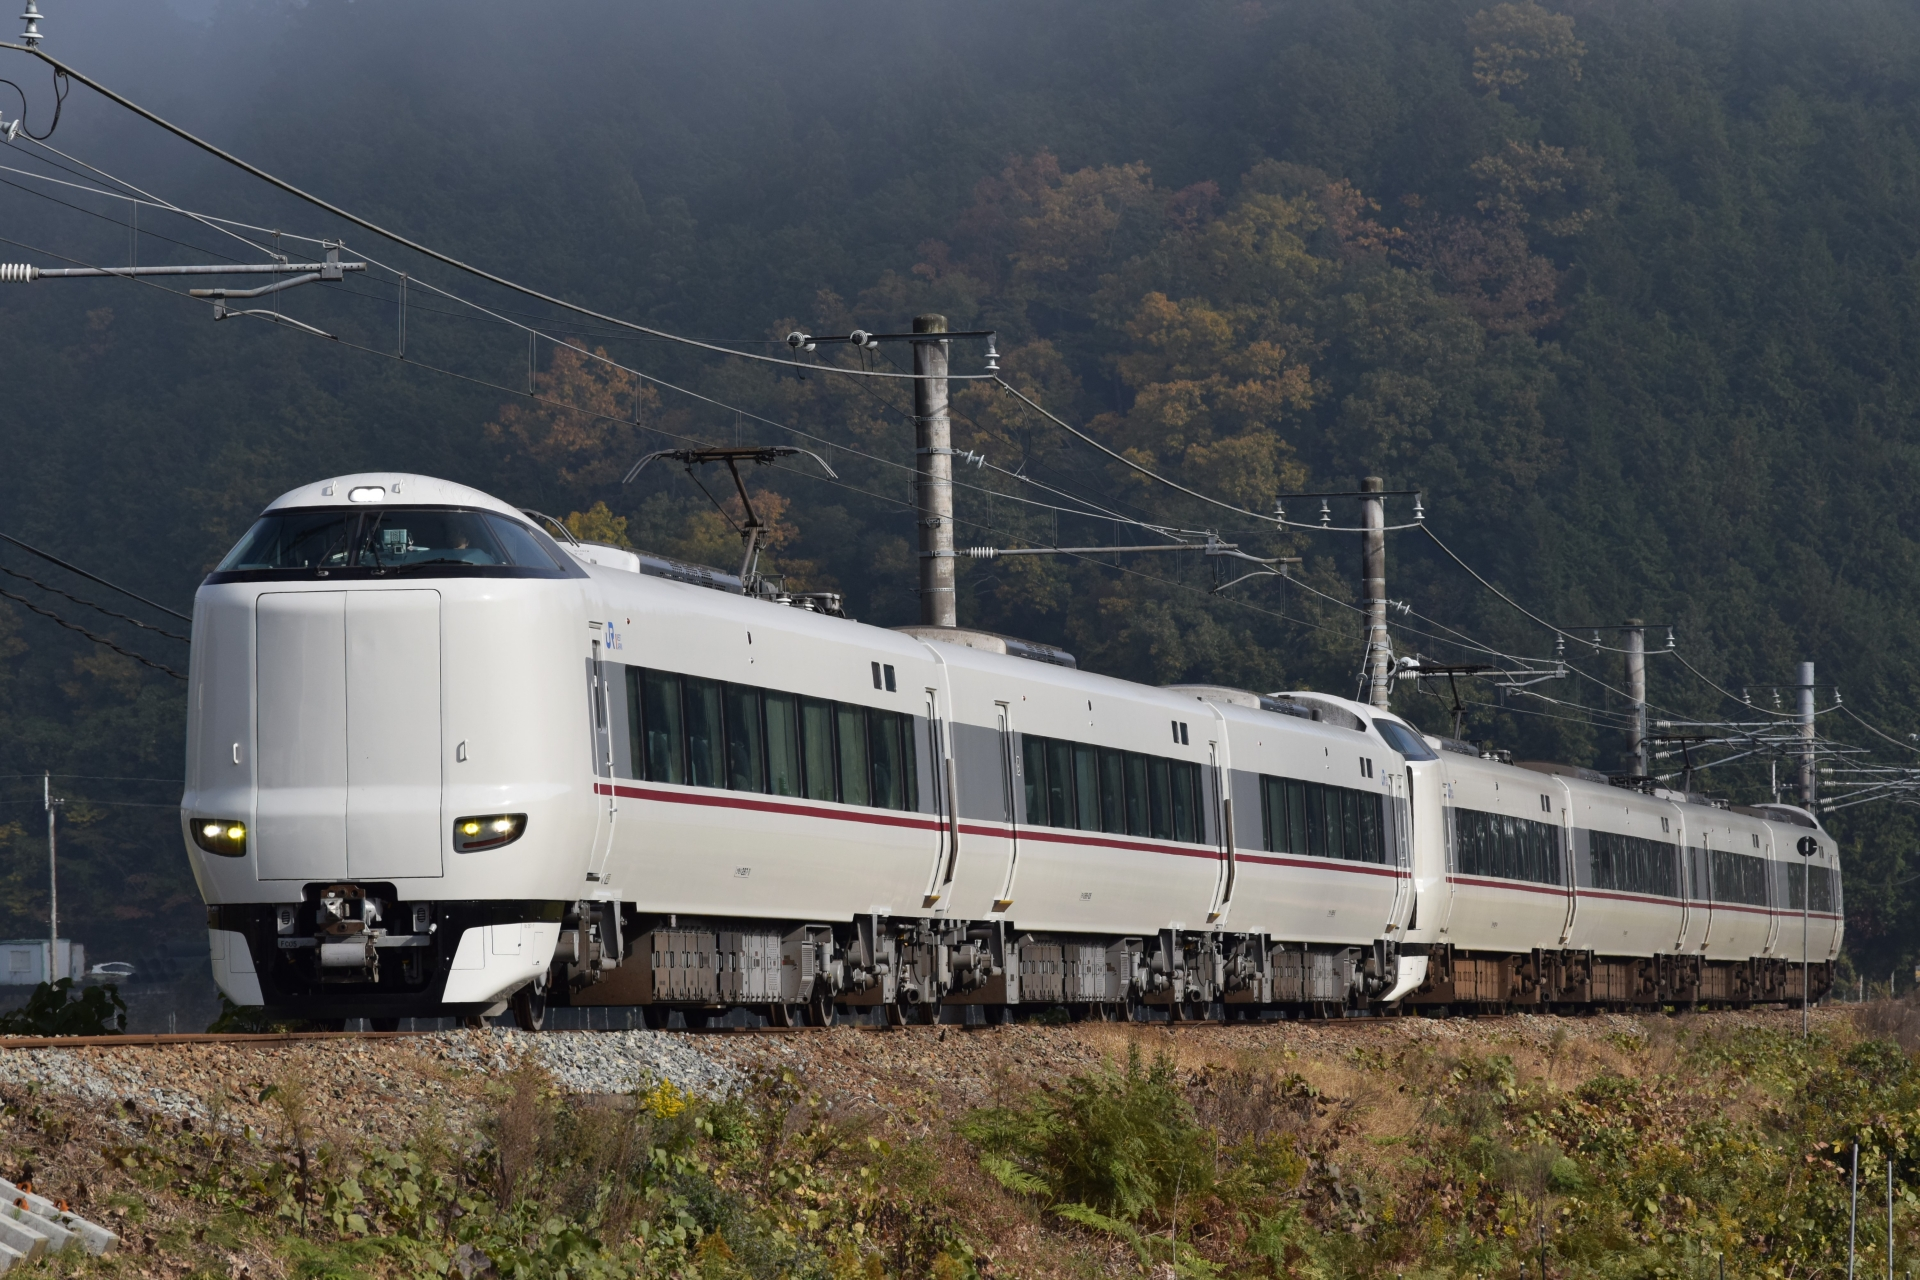
\includegraphics[width=0.7\linewidth]{chap4/fig/287}
	\caption{287系}
	\label{fig:287}
\end{figure}

% TODO: \usepackage{graphicx} required
\begin{figure}
	\centering
	\includegraphics[width=0.7\linewidth]{chap4/fig/683}
	\caption{683系}
	\label{fig:683}
\end{figure}

 % 4章
% !TeX root = paper.tex


\chapter{結論}
本プロジェクトでは,機械学習を用いた電車の車両タイプを判別するシステムの開発を行った.
また,電車が写っている画像や動画をサーバ上で,分類,識別を行い判別結果を出力するWebアプリを作成した.

YouTubeの動画から電車の画像を保存して,トレーニング用とバリデーション用の画像を収集しデータセットを作成した.
そのデータセットとYOLOを用いて,車両タイプの分類モデルと識別モデルの2種類のモデルの作成を行った.
車両タイプを知るためには分類モデルを作成すればよいと考えていたが,分類モデルでは動画に写る電車の車両タイプの判別ができないため,識別モデルを作成した.

%作成したモデルの正解率は車両タイプによって差ができた.JR西日本の在来線の一部の車両タイプについては,短時間で車両タイプを知ることができるようになった.
本システムを利用することで電車の知識がない人でも画像または動画に写る一部の車両タイプが何なのかを知ることができるようになった.


===========ここから田村========== % 5章

% !TeX root = paper.tex


\renewcommand{\bibname}{参考文献}
%\addcontentsline{toc}{chapter}{\protect\numberline{参考文献}}
%\addcontentsline{toc}{chapter}{参考文献}
\begin{thebibliography}{99}
\bibitem{YOLO}"Ultralytics YOLOv8 ドキュメント",\url{https://docs.ultralytics.com/ja}
\bibitem{ac} "PhotoAC 写真素材のフリーサイト",\url{https://www.photo-ac.com/}

 \end{thebibliography}
 
 % 参考文献
\newpage
% !TeX root = paper.tex


\appendix %付録
\chapter{サーバ用プログラム}
リスト\ref{js}はブラウザから画像を受け取り,車両タイプの判別を行い,結果の出力を行うプログラムである.
\lstinputlisting[caption=server.js,label=js]{appendix/src/img_rec_server.js}
\chapter{モデル作成時に使用したプログラム}
\section{使い方}
リスト\ref{project_processing.py}には保存した動画から電車の画像を保存するための関数が定義されている.リスト\ref{save.py}ではリスト\ref{project_processing.py}の関数を利用して画像を保存する.リスト\ref{save.py}を実行する際には引数に保存する画像の枚数と車両タイプを指定してから実行する.

図\ref{downloadApp}で入力されたデータをリスト\ref{forms.py}を使用して受け取る.受け取ったデータをリスト\ref{views.py}に送り,1〜3種類の動画を保存し,連結する.
%%%%%%%%%%%%% プログラムの埋め込み %%%%%%%%%%%%%%%%%%%%%%%%%

\section{ソースコード}
%% ファイル名を指定して、挿入する場合
%\lstinputlisting[language=c,caption=サンプルプログラム,label=sample.c]{appendix/src/sample.c}
%project_processing.pyとsave.py
\lstinputlisting[language=Python,caption=project\_processing.py,label=project_processing.py]{appendix/src/project_processing.py}
\lstinputlisting[language=Python,caption=save.py ,label=save.py]{appendix/src/save.py}

%\Istinputlisting[language=Python,caption=views.py,label=views.py]{appendix/src/views.py}

\lstinputlisting[language=Python,caption=views.py ,label=views.py]{appendix/src/views.py}
\lstinputlisting[language=Python,caption=forms.py ,label=forms.py]{appendix/src/forms.py}

%\lstinputlisting[language=html,caption=input_urls_3.html ,label= input3]{appendix/src/input_urls_3.html}



     % 付録  listingsがうまくイカない

\end{document}
